\documentclass[12pt]{article}
%DIF LATEXDIFF DIFFERENCE FILE


\usepackage[top=1in,left=1in, right = 1in, footskip=1in]{geometry}

\usepackage{graphicx}
\usepackage{xspace}
%\usepackage{adjustbox}

\newcommand{\comment}{\showcomment}
%% \newcommand{\comment}{\nocomment}

\newcommand{\showcomment}[3]{\textcolor{#1}{\textbf{[#2: }\textsl{#3}\textbf{]}}}
\newcommand{\nocomment}[3]{}

\newcommand{\jd}[1]{\comment{cyan}{JD}{#1}}
\newcommand{\swp}[1]{\comment{magenta}{SWP}{#1}}
\newcommand{\bmb}[1]{\comment{blue}{BMB}{#1}}
\newcommand{\djde}[1]{\comment{red}{DJDE}{#1}}

%DIF 19c19
%DIF < \newcommand{\eref}[1]{Eq.~\ref{eq:#1}}
%DIF -------
\newcommand{\eref}[1]{Eq.~(\ref{eq:#1})} %DIF > 
%DIF -------
\newcommand{\fref}[1]{Fig.~\ref{fig:#1}}
\newcommand{\Fref}[1]{Fig.~\ref{fig:#1}}
\newcommand{\sref}[1]{Sec.~\ref{#1}}
\newcommand{\frange}[2]{Fig.~\ref{fig:#1}--\ref{fig:#2}}
\newcommand{\tref}[1]{Table~\ref{tab:#1}}
\newcommand{\tlab}[1]{\label{tab:#1}}
\newcommand{\seminar}{SE\mbox{$^m$}I\mbox{$^n$}R}

\usepackage{amsthm}
\usepackage{amsmath}
\usepackage{amssymb}
\usepackage{amsfonts}

\usepackage{lineno}
\linenumbers

\usepackage[pdfencoding=auto, psdextra]{hyperref}

\usepackage{natbib}
\bibliographystyle{chicago}
\date{\today}

\usepackage{xspace}
\newcommand*{\ie}{i.e.\@\xspace}

\usepackage{color}

\newcommand{\Rx}[1]{\ensuremath{{\mathcal R}_{#1}}\xspace} 
\newcommand{\Ro}{\Rx{0}}
\newcommand{\Rc}{\Rx{\mathrm{c}}}
\newcommand{\RR}{\ensuremath{{\mathcal R}}\xspace}
\newcommand{\Rhat}{\ensuremath{{\hat\RR}}}
\newcommand{\Rintrinsic}{\ensuremath{{\mathcal R}_{\textrm{\tiny intrinsic}}}\xspace}
\newcommand{\tsub}[2]{#1_{{\textrm{\tiny #2}}}}
\newcommand{\dd}[1]{\ensuremath{\, \mathrm{d}#1}}
\newcommand{\dtau}{\dd{\tau}}
\newcommand{\dx}{\dd{x}}
\newcommand{\dsigma}{\dd{\sigma}}

\newcommand{\psymp}{\ensuremath{p}} %% primary symptom time
\newcommand{\ssymp}{\ensuremath{s}} %% secondary symptom time
\newcommand{\pinf}{\ensuremath{\alpha_1}} %% primary infection time
\newcommand{\sinf}{\ensuremath{\alpha_2}} %% secondary infection time

\newcommand{\psize}{{\mathcal P}} %% primary cohort size
\newcommand{\ssize}{{\mathcal S}} %% secondary cohort size

\newcommand{\gtime}{\sigma} %% generation interval
\newcommand{\gdist}{g} %% generation-interval distribution
\newcommand{\idist}{\ell} %% incubation period distribution

\newcommand{\total}{{\mathcal T}} %% total number of serial intervals
%DIF PREAMBLE EXTENSION ADDED BY LATEXDIFF
%DIF UNDERLINE PREAMBLE %DIF PREAMBLE
\RequirePackage[normalem]{ulem} %DIF PREAMBLE
\RequirePackage{color}\definecolor{RED}{rgb}{1,0,0}\definecolor{BLUE}{rgb}{0,0,1} %DIF PREAMBLE
\providecommand{\DIFaddtex}[1]{{\protect\color{blue}\uwave{#1}}} %DIF PREAMBLE
\providecommand{\DIFdeltex}[1]{{\protect\color{red}\sout{#1}}}                      %DIF PREAMBLE
%DIF SAFE PREAMBLE %DIF PREAMBLE
\providecommand{\DIFaddbegin}{} %DIF PREAMBLE
\providecommand{\DIFaddend}{} %DIF PREAMBLE
\providecommand{\DIFdelbegin}{} %DIF PREAMBLE
\providecommand{\DIFdelend}{} %DIF PREAMBLE
%DIF FLOATSAFE PREAMBLE %DIF PREAMBLE
\providecommand{\DIFaddFL}[1]{\DIFadd{#1}} %DIF PREAMBLE
\providecommand{\DIFdelFL}[1]{\DIFdel{#1}} %DIF PREAMBLE
\providecommand{\DIFaddbeginFL}{} %DIF PREAMBLE
\providecommand{\DIFaddendFL}{} %DIF PREAMBLE
\providecommand{\DIFdelbeginFL}{} %DIF PREAMBLE
\providecommand{\DIFdelendFL}{} %DIF PREAMBLE
%DIF HYPERREF PREAMBLE %DIF PREAMBLE
\providecommand{\DIFadd}[1]{\texorpdfstring{\DIFaddtex{#1}}{#1}} %DIF PREAMBLE
\providecommand{\DIFdel}[1]{\texorpdfstring{\DIFdeltex{#1}}{}} %DIF PREAMBLE
\newcommand{\DIFscaledelfig}{0.5}
%DIF HIGHLIGHTGRAPHICS PREAMBLE %DIF PREAMBLE
\RequirePackage{settobox} %DIF PREAMBLE
\RequirePackage{letltxmacro} %DIF PREAMBLE
\newsavebox{\DIFdelgraphicsbox} %DIF PREAMBLE
\newlength{\DIFdelgraphicswidth} %DIF PREAMBLE
\newlength{\DIFdelgraphicsheight} %DIF PREAMBLE
% store original definition of \includegraphics %DIF PREAMBLE
\LetLtxMacro{\DIFOincludegraphics}{\includegraphics} %DIF PREAMBLE
\newcommand{\DIFaddincludegraphics}[2][]{{\color{blue}\fbox{\DIFOincludegraphics[#1]{#2}}}} %DIF PREAMBLE
\newcommand{\DIFdelincludegraphics}[2][]{% %DIF PREAMBLE
\sbox{\DIFdelgraphicsbox}{\DIFOincludegraphics[#1]{#2}}% %DIF PREAMBLE
\settoboxwidth{\DIFdelgraphicswidth}{\DIFdelgraphicsbox} %DIF PREAMBLE
\settoboxtotalheight{\DIFdelgraphicsheight}{\DIFdelgraphicsbox} %DIF PREAMBLE
\scalebox{\DIFscaledelfig}{% %DIF PREAMBLE
\parbox[b]{\DIFdelgraphicswidth}{\usebox{\DIFdelgraphicsbox}\\[-\baselineskip] \rule{\DIFdelgraphicswidth}{0em}}\llap{\resizebox{\DIFdelgraphicswidth}{\DIFdelgraphicsheight}{% %DIF PREAMBLE
\setlength{\unitlength}{\DIFdelgraphicswidth}% %DIF PREAMBLE
\begin{picture}(1,1)% %DIF PREAMBLE
\thicklines\linethickness{2pt} %DIF PREAMBLE
{\color[rgb]{1,0,0}\put(0,0){\framebox(1,1){}}}% %DIF PREAMBLE
{\color[rgb]{1,0,0}\put(0,0){\line( 1,1){1}}}% %DIF PREAMBLE
{\color[rgb]{1,0,0}\put(0,1){\line(1,-1){1}}}% %DIF PREAMBLE
\end{picture}% %DIF PREAMBLE
}\hspace*{3pt}}} %DIF PREAMBLE
} %DIF PREAMBLE
\LetLtxMacro{\DIFOaddbegin}{\DIFaddbegin} %DIF PREAMBLE
\LetLtxMacro{\DIFOaddend}{\DIFaddend} %DIF PREAMBLE
\LetLtxMacro{\DIFOdelbegin}{\DIFdelbegin} %DIF PREAMBLE
\LetLtxMacro{\DIFOdelend}{\DIFdelend} %DIF PREAMBLE
\DeclareRobustCommand{\DIFaddbegin}{\DIFOaddbegin \let\includegraphics\DIFaddincludegraphics} %DIF PREAMBLE
\DeclareRobustCommand{\DIFaddend}{\DIFOaddend \let\includegraphics\DIFOincludegraphics} %DIF PREAMBLE
\DeclareRobustCommand{\DIFdelbegin}{\DIFOdelbegin \let\includegraphics\DIFdelincludegraphics} %DIF PREAMBLE
\DeclareRobustCommand{\DIFdelend}{\DIFOaddend \let\includegraphics\DIFOincludegraphics} %DIF PREAMBLE
\LetLtxMacro{\DIFOaddbeginFL}{\DIFaddbeginFL} %DIF PREAMBLE
\LetLtxMacro{\DIFOaddendFL}{\DIFaddendFL} %DIF PREAMBLE
\LetLtxMacro{\DIFOdelbeginFL}{\DIFdelbeginFL} %DIF PREAMBLE
\LetLtxMacro{\DIFOdelendFL}{\DIFdelendFL} %DIF PREAMBLE
\DeclareRobustCommand{\DIFaddbeginFL}{\DIFOaddbeginFL \let\includegraphics\DIFaddincludegraphics} %DIF PREAMBLE
\DeclareRobustCommand{\DIFaddendFL}{\DIFOaddendFL \let\includegraphics\DIFOincludegraphics} %DIF PREAMBLE
\DeclareRobustCommand{\DIFdelbeginFL}{\DIFOdelbeginFL \let\includegraphics\DIFdelincludegraphics} %DIF PREAMBLE
\DeclareRobustCommand{\DIFdelendFL}{\DIFOaddendFL \let\includegraphics\DIFOincludegraphics} %DIF PREAMBLE
%DIF END PREAMBLE EXTENSION ADDED BY LATEXDIFF

\begin{document}

\DIFdelbegin %DIFDELCMD < \begin{flushleft}{
%DIFDELCMD < 	\Large
%DIFDELCMD < 	\textbf\newline{
%DIFDELCMD < 		Unraveling the paradox between generation and serial intervals
%DIFDELCMD < 	}
%DIFDELCMD < }
%DIFDELCMD < %%%
\DIFdelend \DIFaddbegin \begin{flushleft}{
	\Large
	\textbf\newline{
		Cohort-based approach to understanding the roles of generation and serial intervals in shaping epidemiological dynamics
	}
}
\DIFaddend \newline
\\
Sang Woo Park\textsuperscript{1,*}
Kaiyuan Sun\textsuperscript{2}
Benjamin M.\ Bolker\textsuperscript{3,4,5}
David Champredon\textsuperscript{6}
David J.\,D.\ Earn\textsuperscript{4,5}
Michael Li\textsuperscript{3}
Joshua S.\ Weitz\textsuperscript{7, 8}
Bryan T.\ Grenfell\textsuperscript{1,2,9}
Jonathan Dushoff\textsuperscript{3,4,5}
\\
\bigskip
\textbf{1} Department of Ecology and Evolutionary Biology, Princeton University, Princeton, NJ, USA
\\
\textbf{2} Fogarty International Center, National Institutes of Health, Bethesda, MD, USA
\\
\textbf{3} Department of Biology, McMaster University, Hamilton, ON, Canada
\\
\textbf{4} Department of Mathematics and Statistics, McMaster University, Hamilton, ON, Canada
\\
\textbf{5} M.\,G.\,DeGroote Institute for Infectious Disease Research, McMaster University, Hamilton, ON, Canada
\\
\textbf{6} Department of Pathology and Laboratory Medicine, University of Western Ontario, London, Ontario, Canada
\\
\textbf{7} School of Biological Sciences, Georgia Institute of Technology, Atlanta, GA, USA
\\
\textbf{8} School of Physics, Georgia Institute of Technology, Atlanta, GA, USA
\\
\textbf{9} Woodrow Wilson School of Public and International Affairs, Princeton University, Princeton, NJ, USA
\\
\bigskip

*Corresponding author: swp2@princeton.edu
\DIFaddbegin \bigskip

\DIFadd{Disclaimer: The findings and conclusions in this report are those of the authors and do not necessarily represent the official position of the U.S. National Institutes of Health or Department of Health and Human Services.
}\DIFaddend \end{flushleft}

\pagebreak

\section*{Abstract}

Generation \DIFaddbegin \DIFadd{intervals }\DIFaddend and serial intervals are \DIFdelbegin \DIFdel{under-appreciated yet important }\DIFdelend \DIFaddbegin \DIFadd{critical }\DIFaddend quantities for characterizing \DIFdelbegin \DIFdel{the outset of an outbreak .
Even though their definitions (and differences) were clearly laid out over a decade ago, there is still a need for clear conceptual and theoretical understanding of their roles in shaping the epidemiological dynamics.
Part of the confusion can be attributed to an apparent paradox.
By definition, both generation and serial intervals describe how infection spreads between individuals --- thus, one would expect them both to }\DIFdelend \DIFaddbegin \DIFadd{outbreak dynamics.
Generation intervals characterize the time between infection and transmission; whereas serial intervals characterize the time between the onset of symptoms in a chain of transmission.
They are often used interchangeably, leading to misunderstanding of how to use either generation or serial intervals to establish a }\DIFaddend link between the epidemic growth rate $r$ and the reproduction number \RR.
\DIFdelbegin \DIFdel{However, current theory does not explain how two different distributions can estimate the same }%DIFDELCMD < \RR %%%
\DIFdel{from }\DIFdelend \DIFaddbegin \DIFadd{On one hand, generation intervals provide a mechanistic link between }\DIFaddend $r$ \DIFdelbegin \DIFdel{--- some studies have further demonstrated that generation and serial }\DIFdelend \DIFaddbegin \DIFadd{and }\RR \DIFadd{but are harder to measure via contact tracing.
On the other hand, serial intervals are easier to measure from contact tracing but recent studies suggest that two }\DIFaddend intervals give different estimates of \RR \DIFdelbegin \DIFdel{.
We provide an answer to the paradox by showing }\DIFdelend \DIFaddbegin \DIFadd{from $r$.
We present a general framework for characterizing }\emph{\DIFadd{any}} \DIFadd{epidemiological delays based on cohorts (i.e., a group of individuals that share the same event time, such as symptom onset) and show }\DIFaddend that \emph{forward-looking} serial intervals, which correctly estimates \RR from $r$, are not the same as ``intrinsic'' serial intervals, but instead change with $r$.
We provide a heuristic \DIFdelbegin \DIFdel{way of }\DIFdelend \DIFaddbegin \DIFadd{method for }\DIFaddend addressing potential biases that can arise from not accounting for changes in \DIFdelbegin \DIFdel{these references and apply our framework to serial intervals of }\DIFdelend \DIFaddbegin \DIFadd{serial intervals across cohorts and apply the method to estimating }\RR \DIFadd{for the }\DIFaddend COVID-19 \DIFaddbegin \DIFadd{outbreak in China using serial interval data --- our analysis shows that using incorrectly defined serial intervals can severely bias the estimate}\DIFaddend .
This study demonstrates the importance of early epidemiological investigation through contact tracing \DIFdelbegin \DIFdel{for characterizing initial serial intervals }\DIFdelend and provides rationale for reassessing \DIFaddbegin \DIFadd{generation intervals, }\DIFaddend serial intervals, and \RR\ estimates, for COVID-19.

\section*{Significance}

The generation- and serial-interval distributions are key\DIFaddbegin \DIFadd{, but different, }\DIFaddend quantities in outbreak analyses.
Recent theoretical studies suggest that two distributions give different estimates of \DIFaddbegin \DIFadd{the reproduction number }\DIFaddend \RR \DIFaddbegin \DIFadd{from the exponential growth rate $r$}\DIFaddend ;
however, both intervals, by definition, \DIFdelbegin \DIFdel{can equally describe the }\DIFdelend \DIFaddbegin \DIFadd{describe }\DIFaddend disease transmission at the individual level.
Here, we show that the serial-interval distribution, defined from the correct reference time and cohort, gives the same estimate of \RR as the generation-interval distribution.
We then apply our framework to serial interval data from the COVID-19 \DIFdelbegin \DIFdel{epidemic}\DIFdelend \DIFaddbegin \DIFadd{outbreak in China}\DIFaddend .
While our study supports the use of serial-interval distributions in estimating \RR, it also reveals \DIFdelbegin \DIFdel{several gaps in }\DIFdelend \DIFaddbegin \DIFadd{necessary changes to }\DIFaddend the current understanding and applications of \DIFdelbegin \DIFdel{the }\DIFdelend serial-interval \DIFdelbegin \DIFdel{distributions}\DIFdelend \DIFaddbegin \DIFadd{distribution}\DIFaddend .

\pagebreak

\section{Introduction}

The reproduction number \RR is one of the most important characteristics of an emerging epidemic\DIFdelbegin \DIFdel{such as }\DIFdelend \DIFaddbegin \DIFadd{, including characterization of }\DIFaddend coronavirus disease 2019 (COVID-19) \citep{majumder2020early}.
The reproduction number is defined as the average number of secondary cases caused by a primary case;
the reproduction number in a fully susceptible population --- referred to as the basic reproduction number \Ro --- allows us to predict the extent to which a disease will spread in the population and the amount of intervention necessary to eliminate disease \citep{anderson1991infectious}.
Near the beginning of an outbreak, \RR is often estimated from the observed exponential growth rate using generation- and serial-interval distributions (e.g., \DIFdelbegin \DIFdel{\mbox{%DIFAUXCMD
\cite{du2020serial, jung2020real, li2020early, zhao2020preliminary}}\hspace{0pt}%DIFAUXCMD
}\DIFdelend \DIFaddbegin \DIFadd{\mbox{%DIFAUXCMD
\cite{wallinga2007generation, fraser2009pandemic, hampson2009transmission, chunara2012social, chowell2014west, du2020serial, jung2020real}}\hspace{0pt}%DIFAUXCMD
}\DIFaddend ).

The generation interval is defined as the time between when an individual (infector) is infected and when that individual infects another person (infectee);
the generation-interval distribution determines the relationship between the exponential growth rate $r$ and the reproduction number \RR \citep{anderson1991infectious, ferguson2005strategies, wallinga2007generation}.
Similarly, the serial interval is defined as the time between when an infector and an infectee become \emph{symptomatic} \citep{svensson2007note}.
While serial intervals are similar to generation intervals, previous studies have noted that, in many contexts, serial intervals are expected to have larger variances than generation intervals but have the same mean \citep{svensson2007note,klinkenberg2011correlation,te2013estimating,champredon2018equivalence}\DIFdelbegin \DIFdel{;
some studies further suggested that using serial intervals can give different estimates of }%DIFDELCMD < \RR %%%
\DIFdel{\mbox{%DIFAUXCMD
\citep{britton2019estimation, ganyani2020estimating}}\hspace{0pt}%DIFAUXCMD
}\DIFdelend .

Although these distributions were clearly and distinctly defined over a decade ago \citep{svensson2007note}, 
the need for a better conceptual and theoretical framework for understanding their differences is becoming clearer as the COVID-19 pandemic unfolds.
Researchers continue to rely on both generation and serial intervals to \DIFdelbegin \DIFdel{make inferences about }\DIFdelend \DIFaddbegin \DIFadd{estimate the reproduction number }\RR \DIFadd{of }\DIFaddend COVID-19, \DIFdelbegin \DIFdel{particularly for estimating its }%DIFDELCMD < \RR%%%
\DIFdel{, }\DIFdelend either without making a clear distinction \citep{tempvar,du2020serial,he2020temporal,wu2020nowcasting,zhao2020serial}, or explicitly conflating the two intervals
\citep{anderson2020will,hellewell2020feasibility}.

One source of confusion comes down to an apparent \DIFdelbegin \DIFdel{paradox}\DIFdelend \DIFaddbegin \DIFadd{discrepancy between biological intuition and mathematical theory}\DIFaddend .
When the epidemic is growing exponentially, the spread of infection can be characterized as a ``renewal process'' based on previous incidence of infection, the associated generation-interval distribution, and the average infectiousness of an infected individual.
This renewal formulation allows us to link the exponential growth rate of an epidemic $r$ with its reproduction number \RR using the generation-interval distribution \citep{wallinga2007generation}.
By definition, the serial-interval distribution describes the renewal process between symptomatic cases based on their symptom onset dates;
therefore, \DIFaddbegin \DIFadd{we expect }\DIFaddend both generation- and serial-interval distributions \DIFdelbegin \DIFdel{should }\DIFdelend \DIFaddbegin \DIFadd{to }\DIFaddend give identical estimates of \RR based \DIFaddbegin \DIFadd{on }\DIFaddend the observed epidemic growth rate $r$.
In contexts where the distributions are expected to be different, current theory has no explanation for how they might provide identical estimates of \RR from $r$\DIFdelbegin \DIFdel{(cf. 
\mbox{%DIFAUXCMD
\cite{britton2019estimation}}\hspace{0pt}%DIFAUXCMD
)}\DIFdelend . 
\DIFaddbegin \DIFadd{Some studies have further suggested that using serial intervals can give different estimates of }\RR \DIFadd{\mbox{%DIFAUXCMD
\citep{britton2019estimation, ganyani2020estimating}}\hspace{0pt}%DIFAUXCMD
.
}\DIFaddend 

Here, we resolve this \DIFdelbegin \DIFdel{paradox}\DIFdelend \DIFaddbegin \DIFadd{discrepancy}\DIFaddend , by showing that the relevant interval for the renewal framework is what is called the ``forward'' interval, and that the forward serial (but not generation) interval is affected by the rate of growth $r$ during the exponential-growth phase.
We develop a new framework for understanding serial intervals\DIFaddbegin \DIFadd{, as well as any other epidemiological delays, }\DIFaddend and show that the initial forward serial-interval distribution correctly estimates \RR from $r$.
Conversely, using inaccurately defined serial intervals or failing to account for changes in the observed serial-interval distributions over the course of an epidemic can significantly bias estimates of \RR.
We apply our framework to serial intervals of COVID-19 and lay out several principles to consider in using information about serial intervals and other epidemiological time delays \DIFdelbegin \DIFdel{in the analysis of epidemics}\DIFdelend \DIFaddbegin \DIFadd{to correctly infer the reproduction number during the early stages of an outbreak}\DIFaddend .

\section{Methods}

\subsection{Intrinsic, forward, and backward delay distributions}

\DIFdelbegin \DIFdel{We first begin by describing a general framework for characterizing a distribution of }\DIFdelend \DIFaddbegin \DIFadd{The }\DIFaddend time delays between two epidemiological events \DIFdelbegin \DIFdel{;
these events }\DIFdelend can be defined either within an infected individual (e.g., \DIFaddbegin \DIFadd{incubation period: }\DIFaddend infection and symptom onset of an individual\DIFdelbegin \DIFdel{, the incubation period}\DIFdelend ) or between infected individuals (e.g., \DIFaddbegin \DIFadd{serial interval: }\DIFaddend symptom onsets of an infector and an infectee\DIFdelbegin \DIFdel{, the serial interval}\DIFdelend ).
We can further divide these events into \emph{primary} and \emph{secondary} events.
When we measure an epidemiological time delay within an infected individual (e.g., the incubation period), the primary event is the event that always or usually occurs before the secondary event ---
most epidemiological events that can be observed within an individual have clear direction (e.g., infection and onset of symptoms) but some may not (e.g., onset of infectiousness and onset of symptoms).
When we measure an epidemiological time delay between infected individuals (e.g., the serial interval), 
the primary and secondary events are defined in terms of the direction of transmission:
the primary event refers to the event that occurs in the infector\DIFdelbegin \DIFdel{; again }\DIFdelend \DIFaddbegin \DIFadd{. 
Again, }\DIFaddend some of these delays are always positive (the infector is always infected before the infectee) and some are not (it is possible for the infectee to \DIFdelbegin \DIFdel{report }\DIFdelend \DIFaddbegin \DIFadd{develop }\DIFaddend symptoms before the infector \DIFaddbegin \DIFadd{\mbox{%DIFAUXCMD
\citep{he2020temporal}}\hspace{0pt}%DIFAUXCMD
}\DIFaddend ).

At the individual level, we can define the expected time distribution between a primary and a secondary event for an average infected individual --- we refer to this distribution as the intrinsic distribution.
For example, the intrinsic incubation period distribution describes the expected time distribution from infection to symptom onset of an average infected individual.
Likewise, the intrinsic generation-interval distribution describes the expected time distribution of infectious contacts made by an average infected individual.
However, the intrinsic time distributions are not always equivalent to the corresponding realized time distributions at the population level (i.e., distribution of time between realized primary and secondary events that occur during an epidemic).
For example, an infectious contact \DIFdelbegin \DIFdel{may not result in infection }\DIFdelend \DIFaddbegin \DIFadd{results in infection only }\DIFaddend if the contacted individual \DIFaddbegin \DIFadd{is susceptible (and }\DIFaddend has already been infected\DIFaddbegin \DIFadd{)}\DIFaddend ;
therefore, the realized generation-interval distribution can be different from the intrinsic generation-interval distribution.

At the population level, we model realized time delays between a primary and a secondary event from a cohort perspective.
A primary cohort consists of \emph{all} individuals whose primary event occurred at a given time; 
a secondary cohort is defined similarly based on the secondary events.
For example, when we are measuring incubation periods, a primary cohort consists of all individuals who became infected at time $\psymp$.
Similarly, when we are measuring serial intervals, a primary cohort consists of all \DIFdelbegin \DIFdel{individuals }\DIFdelend \DIFaddbegin \DIFadd{infectors }\DIFaddend who became symptomatic at time $\psymp$.
Then, for each primary cohort at time $\psymp$, we can define the expected time distribution between primary and secondary events.
We refer to this distribution as the forward delay distribution and denote it as $f_\psymp(\tau)$.

Likewise, we define the backward delay distribution $b_\ssymp(\tau)$ for a secondary cohort at time $\ssymp$:
The backward delay distribution describes the time delays between a primary and secondary host given that the secondary event occurred at time $\ssymp$.
For example, the backward incubation period distribution at time $\ssymp$ describes incubation periods for a \emph{cohort} of individuals who became symptomatic at time $\ssymp$.
Likewise, the backward serial-interval distribution at time $\ssymp$ describes serial intervals for a \emph{cohort} of infectees who became symptomatic at time $\ssymp$.

Both forward and backward perspectives
must yield identical \emph{measurement} (e.g., the length of the incubation
period of a given individual is the same whether measured forward from
the time of infection or backward from the time of symptom onset).
Consequently, if we restrict attention to individuals with a given
incubation period, say $\tau$, and we count how many became infected at time $\psymp$
or how many first showed symptoms at time $\ssymp=\psymp+\tau$ then we must obtain
the same number. In general, no matter how delays are distributed, if
$\mathcal P$ and $\mathcal S$ represent the sizes of primary and
secondary cohorts then we must have
\begin{equation}
\psize(\psymp) f_\psymp(\tau) = \ssize(\ssymp) b_\ssymp(\tau) \,.
\label{eq:match}
\end{equation}
Substituting $\psymp=\ssymp-\tau$, it follows that
\begin{equation}
b_\ssymp(\tau)= \frac{\psize(\ssymp-\tau) f_{\ssymp-\tau} (\tau)}{\ssize(\ssymp)}\DIFaddbegin \DIFadd{\,.
}\DIFaddend \label{eq:backward}
\end{equation}
If we are thinking of realized incubation periods, then the left hand side of
this equation is the probability density that an individual
who became symptomatic at time $\ssymp$ had an incubation period of
length $\tau$. From the right hand side, we see that this probability
density depends on how many individuals became infected at time
$\ssymp-\tau$ [$\psize(\ssymp-\tau)$], how many individuals became
symptomatic at time $\ssymp$ [$\ssize(\ssymp)$], and the probability density
that someone who was infected at time $\ssymp-\tau$ became symptomatic at
time $\ssymp$ [$f_{\ssymp-\tau}(\tau)$]. In general, Eq.~\eqref{eq:backward}
shows that the the backward delay distribution at reference time $\ssymp$
[$b_\ssymp(\tau)$] depends not only on the secondary cohort size at time
$\ssymp$ [$\ssize(\ssymp)$], but also on the primary cohort size at the
earlier time $\ssymp-\tau$ [$\psize(\ssymp-\tau)$] and the forward delay
distribution at that earlier time [$f_{\ssymp-\tau}(\tau)$].

There are multiple mechanisms that drive the changes in forward and backward delay distributions over time.
Typically, within-individual forward delay distributions are not affected by epidemic dynamics.
Some \DIFaddbegin \DIFadd{realized distributions}\DIFaddend , like incubation \DIFdelbegin \DIFdel{periods}\DIFdelend \DIFaddbegin \DIFadd{period distributions}\DIFaddend , are expected to be equivalent to their intrinsic distributions and remain invariant over the course of an epidemic.
\DIFdelbegin \DIFdel{Others}\DIFdelend \DIFaddbegin \DIFadd{Other realized distributions}\DIFaddend , like the \DIFaddbegin \DIFadd{distribution of }\DIFaddend time from symptom onset to testing, may change over the course of an epidemic due to changes in public health policies.
Between-individual forward delay distributions, such as generation- or serial-interval distributions, depend on epidemic dynamics;
for example, forward generation intervals contract during the outbreak because infected individuals are less likely to infect others later due to susceptible depletion \citep{champredon2015intrinsic}.

\eref{backward} suggests that backward delay distributions change over time even if their corresponding forward delay distribution does not change:
Backward delay distributions depend on changes in the primary cohort size over time due to conditionality of observations (i.e., they are measured from a cohort of individuals whose secondary events occurred at the same time).
When the cohort size is increasing (or decreasing) over time, we are biased to observe shorter (or longer) delays when we look backward.
In particular, when the incidence is growing exponentially, we can calculate the amount of bias exactly.
Assuming that the forward delay distribution remains constant during the exponential growth phase (\DIFdelbegin \DIFdel{$\tsub{f}{exp}$}\DIFdelend \DIFaddbegin \DIFadd{$f_p(\tau) \approx f_0(\tau)$}\DIFaddend ), we \DIFdelbegin \DIFdel{have:
}\DIFdelend \DIFaddbegin \DIFadd{can substitute $\psize(t) = \psize(0) \exp(rt)$ in \eref{backward} to obtain:
}\DIFaddend \begin{equation}
\DIFdelbegin %DIFDELCMD < \tsub{b}{exp}%%%
\DIFdelend \DIFaddbegin \DIFadd{b_0}\DIFaddend (\tau) \propto \exp(-r\tau) \DIFdelbegin %DIFDELCMD < \tsub{f}{exp}%%%
\DIFdelend \DIFaddbegin \DIFadd{f_0}\DIFaddend (\tau),
\label{eq:backexp}
\end{equation}
where $r$ is the exponential growth rate.
For faster epidemic (higher $r$), the backward delay distributions will be shorter.
Changes in the backward delay distributions are also affected by the changes in the forward delay distributions by definition (\eref{backward}).
Therefore, the backward delay distributions will be generally different from the forward delay distributions even if we are measuring time delays that are intrinsic to life history of a disease (e.g., incubation period).
These ideas apply to all epidemiological delay distributions and generalize the work by \cite{champredon2015intrinsic} who compared forward and backward generation-interval distributions to describe the realized generation intervals from the perspective of an infector and an infectee, respectively, as well as the work by \cite{britton2019estimation} who showed that \eref{backexp} holds for the backward generation-interval distributions.

\subsection{Realized serial interval distributions}

The serial interval is defined as the time between when an infector becomes symptomatic and when an infectee becomes symptomatic \citep{svensson2007note}.
Previous studies have often expressed serial intervals $\tau$ in the form (\fref{diagram}A):
\begin{equation}
\tau = (\gtime + x\DIFdelbegin \DIFdel{_1}\DIFdelend \DIFaddbegin \DIFadd{_2}\DIFaddend ) - x\DIFdelbegin \DIFdel{_0
}\DIFdelend \DIFaddbegin \DIFadd{_1
}\DIFaddend \end{equation}
where \DIFdelbegin \DIFdel{$x_0$ and }\DIFdelend $x_1$ \DIFaddbegin \DIFadd{and $x_2$ }\DIFaddend represent incubation periods of an infector and an infectee, respectively, and $\gtime$ represents the generation interval.
These studies assumed that \DIFdelbegin \DIFdel{$x_0$ and }\DIFdelend $x_1$ \DIFaddbegin \DIFadd{and $x_2$ }\DIFaddend follow the same distributions and concluded that the serial and generation intervals have the same mean \citep{svensson2007note,klinkenberg2011correlation,champredon2018equivalence, britton2019estimation};
however, this conclusion is based on the implicit assumption that incubation times, \DIFdelbegin \DIFdel{$x_0$ and }\DIFdelend $x_1$ \DIFaddbegin \DIFadd{and $x_2$}\DIFaddend , as well as generation interval, $\gtime$, are intrinsic to individuals (and not dependent on disease dynamics) --- something that is true of forward but not backward incubation times.
We refer to this definition as the intrinsic serial interval \DIFaddbegin \DIFadd{(\fref{diagram}A)}\DIFaddend .

\begin{figure}[!th]
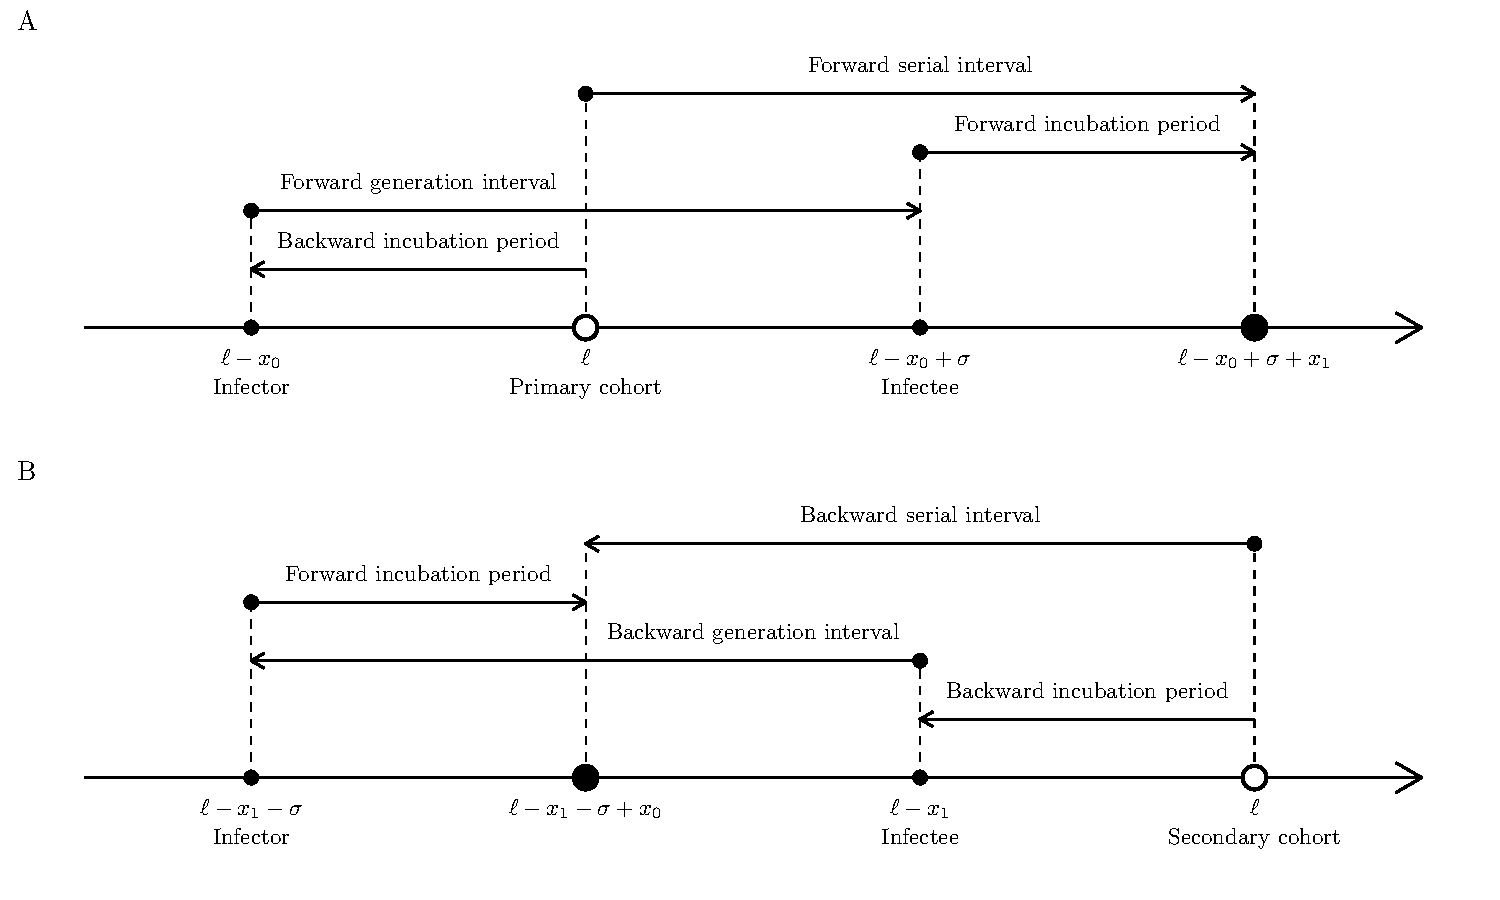
\includegraphics[width=\textwidth]{serial_guide.pdf}
\caption{
\textbf{Illustration of intrinsic, forward and backward serial intervals.}
(A) The intrinsic serial interval for a cohort of individuals infected at time $\psymp$.
In this case, \DIFdelbeginFL \DIFdelFL{$x_0$ }\DIFdelendFL \DIFaddbeginFL \DIFaddFL{$x_1$ }\DIFaddendFL follows the intrinsic incubation period distribution;
$\gtime$ follows the intrinsic generation-interval distribution;
and \DIFdelbeginFL \DIFdelFL{$x_1$ }\DIFdelendFL \DIFaddbeginFL \DIFaddFL{$x_2$ }\DIFaddendFL follows the intrinsic incubation period distribution.
(B) The forward serial interval for a cohort of infectors who became symptomatic at time $\psymp$.
In this case, \DIFdelbeginFL \DIFdelFL{$x_0$ }\DIFdelendFL \DIFaddbeginFL \DIFaddFL{$x_1$ }\DIFaddendFL follows the backward incubation period distribution;
$\gtime$ follows the forward generation-interval distribution;
and \DIFdelbeginFL \DIFdelFL{$x_1$ }\DIFdelendFL \DIFaddbeginFL \DIFaddFL{$x_2$ }\DIFaddendFL follows the forward incubation period distribution.
(C) The backward serial interval for a cohort of infectees who became symptomatic at time $\ssymp$.
In this case, \DIFdelbeginFL \DIFdelFL{$x_0$ }\DIFdelendFL \DIFaddbeginFL \DIFaddFL{$x_1$ }\DIFaddendFL follows the forward incubation period distribution;
$\gtime$ follows the backward generation-interval distribution;
and \DIFdelbeginFL \DIFdelFL{$x_1$ }\DIFdelendFL \DIFaddbeginFL \DIFaddFL{$x_2$ }\DIFaddendFL follows the backward incubation period distribution.
}
\label{fig:diagram}
\end{figure}

To correctly link realized serial intervals to the renewal process between cases based on symptom onset dates, we must use the forward serial interval (i.e., use the perspective of a cohort of infectors that share the same symptom onset time). 
Given that an infector became symptomatic at time $\psymp$, to calculate the forward serial interval we first go backward in time by asking when the infector was infected, and then go forward in time by asking first when the infectee was infected and then when they became symptomatic.
In \fref{diagram}B, we see that \DIFdelbegin \DIFdel{$x_0$ }\DIFdelend \DIFaddbegin \DIFadd{$x_1$ }\DIFaddend follows the backward incubation period distribution of the cohort of infectors who became symptomatic at time $\psymp$;
$\gtime$ follows the forward generation-interval distribution of the cohort of infectors who came infected at time \DIFdelbegin \DIFdel{$\psymp - x_0$;
and $x_1$ }\DIFdelend \DIFaddbegin \DIFadd{$\psymp - x_1$;
and $x_2$ }\DIFaddend follows the forward incubation period distribution of the cohort of infectees who became infected at time \DIFdelbegin \DIFdel{$\psymp - x_0 + \gtime$}\DIFdelend \DIFaddbegin \DIFadd{$\psymp - x_1 + \gtime$}\DIFaddend .
Likewise, we can define the backward serial interval distribution for a cohort of infectees who became symptomatic at time $\ssymp$ (\fref{diagram}C).
This conceptual framework clearly demonstrates that the distributions of \DIFdelbegin \DIFdel{$x_0$, $\ssymp$, and $x_1$ }\DIFdelend \DIFaddbegin \DIFadd{$x_1$, $\gtime$, and $x_2$ }\DIFaddend (and therefore the distributions of realized serial intervals) depend on the reference cohort and the corresponding cohort time.

To calculate realized serial-interval distributions, we begin by modeling $\total(\psymp,\ssymp)$: the total number of serial intervals that start (when infectors develop symptoms) at time $\psymp$ and end (when infectees develop symptoms) at time $\ssymp$.
The number of serial intervals between time $\psymp$ and $\ssymp$, given that the infectors became infected at time $\pinf$ and the infectees became infected at time $\sinf$, depends on the amount of infection that occur between time $\pinf$ and $\sinf$ as well as the densities of forward incubation periods between $\pinf$ and $\psymp$ (realized incubation periods of infectors) as well as $\sinf$ and $\ssymp$ (realized incubation periods of infectees):
\begin{equation}
\underbrace{\Rc (\pinf)}_{\substack{\text{case} \\ \text{reproduction} \\ \text{number}}} 
\times 
\underbrace{i(\pinf)}_{\text{incidence}} 
\times 
\underbrace{h_{\pinf}(\psymp-\pinf, \sinf - \pinf)}_{\substack{\text{joint density of} \\ \text{the forward incubation} \\ \text{period } p-\pinf \text{ and the forward} \\ \text{generation interval } \sinf-\pinf\\ \text{(of infectors)}}}
\times
\underbrace{\idist_{\sinf}(\ssymp - \sinf)}_{\substack{\text{marginal density of} \\ \text{the forward incubation} \\ \text{period } \ssymp-\sinf \\ \text{(of infectees)}}},
\end{equation}
where the case reproduction number $\Rc (\pinf)$ is defined as the average number of secondary cases caused by a primary case infected at time $\pinf$ over the course of their infection \citep{fraser2007estimating}.
We note that it is necessary to describe the forward incubation periods and the forward generation intervals using a joint probability distribution because onset of symptoms and transmission potential jointly depend on the life history of a disease;
for example, if an infected individual can only transmit the disease after symptom onset, the forward generation interval will necessarily be longer than the forward incubation period.

The total number of serial intervals can now be obtained by integrating over all possible infection times for the infector and the infectee:
\begin{equation}
\total (\psymp,\ssymp) = \int_{-\infty}^{\psymp} \int_{\pinf}^{\ssymp} \Rc (\pinf) i(\pinf) h_{\pinf}(\psymp-\pinf, \sinf - \pinf) \idist_{\sinf}(\ssymp - \sinf) \, \mathrm{d}\sinf\,\mathrm{d}\pinf.
\end{equation}
Then, the forward serial-interval distribution $f_\psymp(\tau)$ is given by the density of intervals of length $\tau$ starting at \psymp, relative to the total number of serial intervals starting at \psymp: 
\begin{equation}
f_\psymp(\tau) = 
\DIFdelbegin \DIFdel{\frac{\total(\psymp, \psymp+\tau)}{\int \total(\psymp, \psymp+\tau') d\tau'}}\DIFdelend \DIFaddbegin \DIFadd{\frac{\total(\psymp, \psymp+\tau)}{\int \total(\psymp, \psymp+\tau') \dtau'}}\DIFaddend .
\DIFaddbegin \label{eq:fserial}
\DIFaddend \end{equation}
Likewise, the backward serial-interval distribution $b_\ssymp(\tau)$ is given by the density of intervals of length $\tau$ ending at \ssymp, relative to the total number of serial intervals ending at \ssymp: 
\begin{equation}
b_\ssymp(\tau) = 
\DIFdelbegin \DIFdel{\frac{\total(\ssymp-\tau, \ssymp)}{\int \total(\ssymp-\tau', \ssymp) d\tau'}}\DIFdelend \DIFaddbegin \DIFadd{\frac{\total(\ssymp-\tau, \ssymp)}{\int \total(\ssymp-\tau', \ssymp) \dtau'}}\DIFaddend .
\DIFaddbegin \label{eq:bserial}
\DIFaddend \end{equation}
\DIFaddbegin \DIFadd{This framework allows us to understand changes in the realized serial intervals for any deterministic epidemic models.
}\DIFaddend 

\subsection{Epidemic model}

We illustrate \DIFdelbegin \DIFdel{the theory }\DIFdelend \DIFaddbegin \DIFadd{changes in the forward and backward serial intervals over the course of an epidemic }\DIFaddend by applying it to a specific example of an epidemic model. 
We model disease spread with a renewal-equation model \citep{heesterbeek1996concept, diekmann2000mathematical, roberts2004modelling, aldis2005integral, roberts2007model, champredon2018equivalence}.
Ignoring births and deaths, changes in the proportion of susceptible individuals $S(t)$ and incidence of infection $i(t)$ can be written as:
\begin{equation}
\begin{aligned}
\frac{\mathrm{d}S}{\mathrm{d}t} &= - i(t)\\
i(t) &= \Ro S(t) \int_0^\infty i(t-\tau) \gdist(\tau) \dtau,
\end{aligned}
\label{eq:renewal}
\end{equation}
where \Ro is the basic reproduction number, and $\gdist(\tau)$ is the intrinsic generation-interval distribution (i.e., the forward generation-interval distribution of a primary case in a population where the number of susceptibles remains constant).
Then, the forward generation-interval for a cohort of individuals that were infected at time $\psymp$ follows \citep{champredon2015intrinsic}:
\begin{equation}
\gdist_\psymp (\tau) \propto \gdist(\tau) S(\psymp + \tau),
\end{equation}
which allows us to separate the joint probability distribution $h_\psymp$ of the forward incubation period and the forward generation-interval distribution as a product of the proportion of susceptible individuals $S$ and the joint probability distribution $h$ of the forward incubation period and the intrinsic generation intervals:
\begin{equation}
h_\psymp (x, \tau) \propto h(x, \tau) S(\psymp + \tau).
\end{equation}
We further assume that the forward incubation period distributions does not vary across cohorts over the course of an epidemic, as they represent the life history of a disease, and use \DIFdelbegin \DIFdel{$k$ }\DIFdelend \DIFaddbegin \DIFadd{$\idist$ }\DIFaddend without subscript instead. 
Then, we have:
\begin{equation}
\begin{aligned}
\idist(x) &= \int_0^\infty h(x, \tau) \dtau\\
\gdist(\tau) &= \int_0^\infty h(x, \tau) \dx
\end{aligned}
\end{equation}
Finally, the case reproduction for this model is defined as follows:
\begin{equation}
\Rc(t) = \Ro \int_0^\infty \gdist(\tau) S(t+\tau) \dtau.
\end{equation}
\DIFdelbegin %DIFDELCMD < 

%DIFDELCMD < %%%
\DIFdelend \DIFaddbegin \DIFadd{The forward and backward serial-interval distributions are then calculated by substituting these quantities into \eref{fserial} and \eref{bserial}.
}\DIFaddend We use this framework to illustrate how the realized epidemiological time distributions vary over the course of an epidemic and depend on the perspective.
\DIFdelbegin \DIFdel{We run deterministic as well as stochastic simulations based on the renewal equations (see Appendix) using previously estimated intrinsic incubation period and intrinsic generation-interval distributions for COVID-19 (Table 1) and compare both the forward and backward delay distributions;
in particular, we focus on the realized incubation period, generation-interval, and serial-interval distributions.
}\DIFdelend 

\subsection{Linking $r$ and \RR}

During the initial phase of an epidemic, the proportion susceptible remains approximately constant ($S(t) \approx S(0)$) and incidence of infection grows exponentially: $i(t)=i_0\exp(rt)$.
During this period, the intrinsic generation-interval distribution provides the correct link between the exponential growth rate $r$ and the initial reproduction number $\RR=\Ro S(0)$ based on the Euler-Lotka equation \citep{wallinga2007generation};
in this case, we focus on the estimates of the basic reproduction number \Ro (the value of \RR in a fully susceptible population, $S(t) \approx 1$):
\begin{equation}
\frac{1}{\Ro} = \int_0^\infty \exp(-r\tau) g(\tau) \dtau.
\DIFaddbegin \label{eq:Rgen}
\DIFaddend \end{equation}
Analogous to the intrinsic generation-interval distribution, 
forward serial-interval distributions, by definition, describe the renewal process of infection based on symptom onset dates.
Therefore, we expect the forward serial-interval distribution during the exponential growth phase --- which we refer to as the \emph{initial} forward serial-interval distribution $f_0$ --- to estimate the same value of \Ro for a given $r$ as the intrinsic generation-interval distribution (note, however, that the forward serial interval is not necessarily positive):
\begin{equation}
\frac{1}{\Ro} = \int_{-\infty}^\infty \exp(-r\tau) f_{0}(\tau) \mathrm{d} \tau,
\DIFaddbegin \label{eq:Rforward}
\DIFaddend \end{equation}
where the initial forward serial-interval distribution is given by:
\begin{equation}
f_{0}(\tau) \propto \int_{-\infty}^{0} \int_{\pinf}^{\tau} \exp(r \pinf) h(-\pinf, \sinf - \pinf) \idist(\tau - \sinf) \, \mathrm{d}\sinf\,\mathrm{d}\pinf.
\DIFaddbegin \label{eq:initialSI}
\DIFaddend \end{equation}
In \DIFdelbegin \DIFdel{the Appendix}\DIFdelend \DIFaddbegin \DIFadd{Supplementary Materials}\DIFaddend , we provide a mathematical proof of this relationship.
We further compare this with the estimate of \Ro based on the intrinsic serial-interval distribution \DIFdelbegin \DIFdel{:
}\DIFdelend \DIFaddbegin \DIFadd{$q(\tau)$:
}\DIFaddend \begin{equation}
\frac{1}{\Rintrinsic} = \int_{-\infty}^\infty \exp(-r\tau) q(\tau) \mathrm{d} \tau,
\DIFaddbegin \label{eq:Rintrinsic}
\DIFaddend \end{equation}
where the intrinsic serial-interval distribution \DIFaddbegin \DIFadd{$q(\tau)$ }\DIFaddend does not depend on disease dynamics:
\begin{equation}
q(\tau) \propto \int_{-\infty}^{0} \int_{\pinf}^{\tau} h(-\pinf, \sinf - \pinf) \idist(\tau - \sinf) \, \mathrm{d}\sinf\,\mathrm{d}\pinf.
\DIFaddbegin \label{eq:intrinsicSI}
\DIFaddend \end{equation}
\DIFaddbegin \DIFadd{Instead of numerically integrating over closed forms of $g$, $f_0$, and $q$ to estimate $\Ro$, we use simulation-based approaches for simplicity (Supplementary Materials).
}\DIFaddend 

The initial forward serial-interval distribution depends on the exponential growth rate $r$.
For a fast-growing epidemic (high $r$), we expect the backward incubation periods to be short (\eref{backexp}), and therefore, the forward serial-interval distribution will generally have a larger mean than the intrinsic generation- and serial-interval distributions.
The Susceptible-Exposed-Infected-Recovered model, with an additional assumption that incubation and exposed periods are equivalent, provides a special case where the forward serial- and generation-intervals follow the same distributions during the exponential growth phase because (i) infected individuals can only transmit after symptom onset and (ii) the time between symptom onset to infection is independent of the incubation period of an infector (see \DIFdelbegin \DIFdel{Appendix}\DIFdelend \DIFaddbegin \DIFadd{Supplementary Materials}\DIFaddend ).

\begin{table}[!th]
\begin{center}
\begin{tabular}{|l|l|r|}
\hline
Parameter & Values & Source\\
\hline
Mean \DIFdelbeginFL \DIFdelFL{forward }\DIFdelendFL \DIFaddbeginFL \DIFaddFL{intrinsic }\DIFaddendFL incubation period & 5.5 days & \cite{lauer2020incubation} \\
SD \DIFdelbeginFL \DIFdelFL{forward }\DIFdelendFL \DIFaddbeginFL \DIFaddFL{intrinsic }\DIFaddendFL incubation period & 2.4 days & \cite{lauer2020incubation} \\
Mean intrinsic generation interval & 5 days & \cite{ferretti2020quantifying} \\
SD intrinsic generation interval & 2 days & \cite{ferretti2020quantifying} \\
\hline
\end{tabular}
\end{center}
\caption{
\textbf{Parameter values used for simulations.}
The intrinsic generation-interval distribution is parameterized using a log-normal distribution with log mean $\mu_G=1.54$ and log standard deviation $\sigma_G=0.37$.
The forward incubation period distribution is parameterized using a log-normal distribution with log mean $\mu_I=1.62$ and log standard deviation $\sigma_I=0.42$.
The joint probability distribution is modeled using a multivariate log-normal distribution with correlations (on the log scale) $\rho=-0.5, 0, 0.5$.
}
\end{table}

\section{Results}

\subsection{Realized serial interval distributions}

\DIFaddbegin \DIFadd{First, we compare the estimates of the basic reproduction number }\Ro \DIFadd{based on the initial forward serial-interval distributions and the intrinsic serial-interval distributions (see Supplementary Materials for calculation details.).
In particular, we model the joint probability distribution of the intrinsic incubation periods and generation intervals using a bivariate lognormal distribution with correlation $\rho$ based on parameter estimates for COVID-19 (Table 1).
}\DIFaddend The initial forward serial-interval distributions $f_0(\tau)$ and the intrinsic generation-interval distribution $\gdist(\tau)$ give identical estimates of \Ro \DIFaddbegin \DIFadd{(see \eref{Rgen} and \eref{Rforward}) }\DIFaddend regardless of the correlation $\rho$ between the \DIFdelbegin \DIFdel{forward incubation period distribution }\DIFdelend \DIFaddbegin \DIFadd{intrinsic incubation period }\DIFaddend and the intrinsic \DIFdelbegin \DIFdel{generation-interval distribution }\DIFdelend \DIFaddbegin \DIFadd{generation interval }\DIFaddend (\fref{rR}A).
However, using the intrinsic serial-interval distributions that do not account for disease dynamics (i.e., assuming that the backward and the forward incubation period distributions are identical) underestimates \Ro \DIFaddbegin \DIFadd{(see \eref{Rintrinsic})}\DIFaddend ;
as $r$ increases, \Rintrinsic saturates and eventually decreases due to negative serial intervals (\fref{rR}B).
While the forward serial intervals during the exponential growth phase can also be negative, the proportion of negative intervals are appropriately balanced because faster epidemic growth will lead to shorter backward incubation periods (and therefore a lower proportion of negative serial intervals).

\begin{figure}[!th]
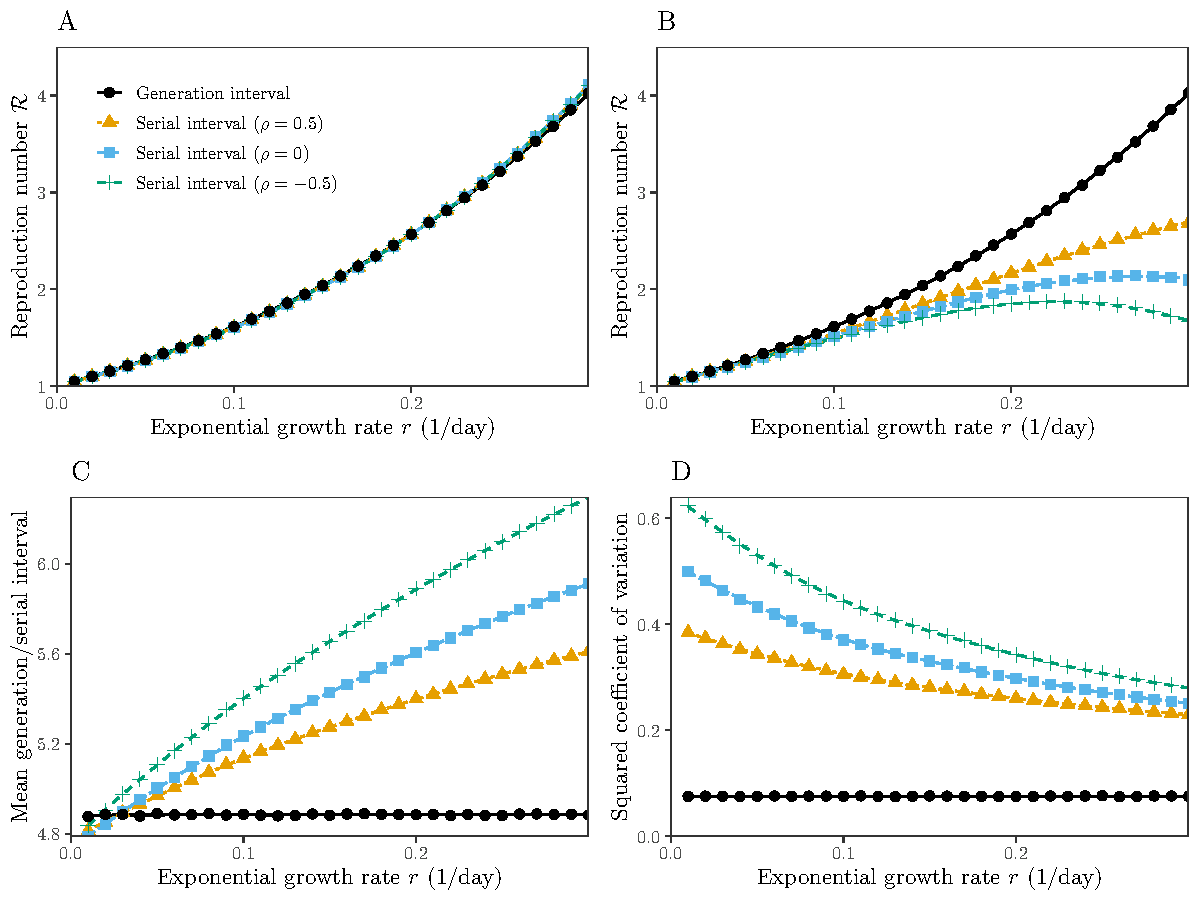
\includegraphics[width=\textwidth]{rR.pdf}
\caption{
\textbf{Estimates of the reproduction number from the exponential growth rate based on serial- and generation-interval distributions.}
(A). The initial forward serial-interval distributions give a correct link between the exponential growth rate $r$ and the reproduction number \Ro.
(B) The intrinsic serial-interval distributions give an incorrect link between $r$ and \Ro.
(C) The mean initial forward serial interval during the exponential growth phase increases with $r$.
(D) The squared coefficient of variation of the initial forward serial intervals during the exponential growth phase decreases with $r$.
}
\label{fig:rR}
\end{figure}

Comparing the shapes of initial forward serial-interval distributions \DIFaddbegin \DIFadd{(\eref{initialSI}) }\DIFaddend and the intrinsic generation-interval distribution allows us to better understand how different forward distributions lead to identical estimates of \Ro.
In general, distributions with higher means and less variability give higher \Ro for a given $r$ \DIFdelbegin \DIFdel{\mbox{%DIFAUXCMD
\citep{wallinga2007generation, park2019practical}}\hspace{0pt}%DIFAUXCMD
}\DIFdelend \DIFaddbegin \DIFadd{\mbox{%DIFAUXCMD
\citep{wallinga2007generation, weitz2015modeling, park2019practical}}\hspace{0pt}%DIFAUXCMD
}\DIFaddend .
When incidence is growing exponentially, forward serial intervals have higher means (\fref{rR}C) and squared coefficients of variation (\fref{rR}D) than the intrinsic generation-interval distribution.
The effects of higher means (which increases \Ro) exactly cancel those of higher variability (which decreases \Ro).
On the other hand, \emph{intrinsic} serial intervals \DIFaddbegin \DIFadd{(\eref{intrinsicSI}) }\DIFaddend have the same mean (equal to the mean initial forward serial at $r=0$ in \fref{rR}C) as the intrinsic generation intervals but are wider (also see squared coefficient of variation of the initial forward serials at $r=0$ in \fref{rR}D); 
therefore, we underestimate \Ro when we use the intrinsic serial-interval distribution.

\begin{figure}[!ht]
\begin{center}
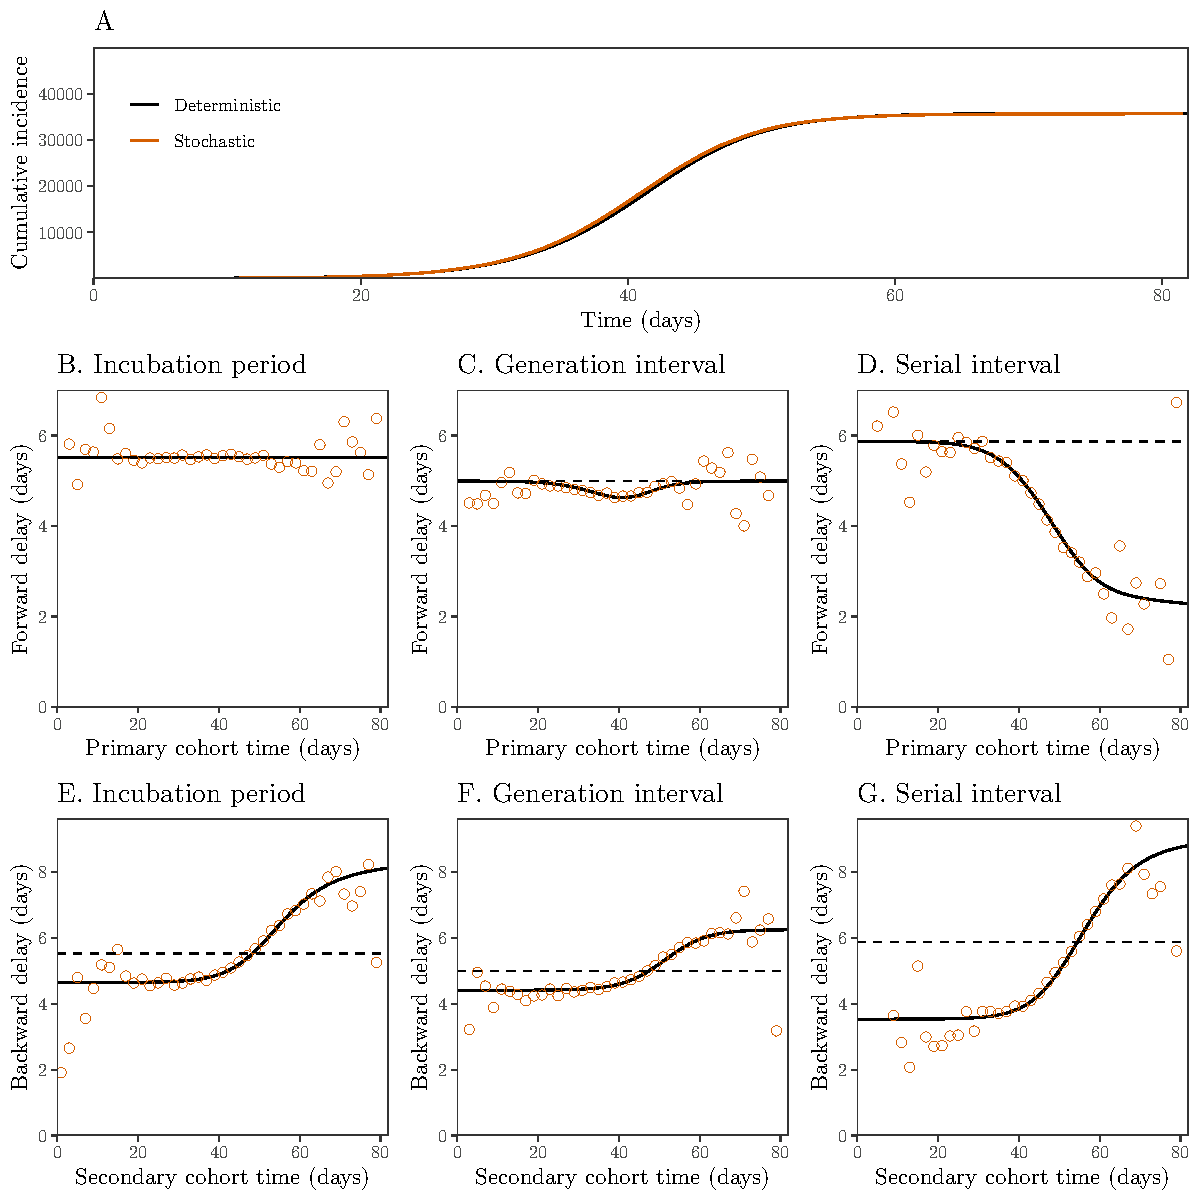
\includegraphics[width=0.95\textwidth]{forward.pdf}
\caption{
\textbf{Epidemiological dynamics and changes in mean forward and backward delay distributions.}
(A) Daily incidence over time.
(B--D) Changes in the mean forward incubation period, generation interval, and serial interval.
(E--G) Changes in the mean backward incubation period, generation interval, and serial interval.
Black lines represent the results of a deterministic simulation.
Orange lines (A) represent the results of 10 stochastic simulations.
Orange points (B-G) represent the average of 10 stochastic simulations.
Dashed lines represent the mean initial forward delay.
Intrinsic incubation periods and intrinsic generation-intervals are assumed to be independent of each other.
See Table 1 for parameter values.
}
\label{fig:epi}
\end{center}
\end{figure}

The initial forward serial interval distribution captures the exponential growth phase of an epidemic.
\DIFdelbegin \DIFdel{Now}\DIFdelend \DIFaddbegin \DIFadd{Next}\DIFaddend , we characterize how forward and backward serial intervals vary over the course of an epidemic \DIFaddbegin \DIFadd{by running deterministic as well as stochastic simulations based on the renewal equations (see Supplementary Materials) using parameters in Table 1;
we further assume $\Ro=2.5$}\DIFaddend .
While the forward serial-interval distribution is our primary focus, understanding the differences between the forward and the backward distributions are important because the observed intervals during on ongoing epidemic are \DIFdelbegin \DIFdel{like backward distributions}\DIFdelend \DIFaddbegin \DIFadd{often the backward ones}\DIFaddend :
we typically identify infected individuals and ask when they were infected by whom.
Similarly, when we are estimating the incubation period of an individual, we often observe their symptom onset date of infected individuals and try to estimate when they were infected (e.g., \cite{backer2020incubation}).

\fref{epi} compares the epidemiological dynamics (A) with the mean forward (B--D) and the mean backward (E--F) delay distributions of a deterministic model based on the renewal equation (\eref{renewal}) and of the corresponding stochastic realizations based on individual-based simulations.
The mean forward incubation period remains constant throughout an epidemic as assumed (\fref{epi}B).
The mean forward generation interval decreases slightly as incidence rate increases, causing the proportion of susceptible population to decrease (\fref{epi}C; \cite{kenah2008generation, champredon2015intrinsic}).
In contrast, the mean forward serial interval decreases over time (\fref{epi}D).

The forward serial interval distributions depend on three intervals (\fref{diagram}): (i) the backward incubation period distributions, (ii) the forward generation-interval distributions, and (iii) the forward incubation period distributions.
For COVID-19 parameters (Table 1), both forward incubation period (\fref{epi}B) and generation-interval (\fref{epi}C) distributions remain roughly constant;
therefore, changes in the forward serial-interval distributions are predominantly driven by changes in the backward incubation period distributions, whose mean increases over time (\fref{epi}D).
In this case, the increase in the mean backward incubation period directly translates to the decrease in the mean forward serial interval.
\DIFdelbegin \DIFdel{Since the increase in the mean backward period is driven by the decreasing incidence, which can still occur in the absence of significant depletion of the susceptible pool via intervention, decrease in the mean forward serial interval may be a robust feature in COVID-19 outbreaks.
}\DIFdelend %DIF >  Since the increase in the mean backward period is driven by the decreasing incidence, which can still occur in the absence of significant depletion of the susceptible pool via intervention, decrease in the mean forward serial interval may be a robust feature in COVID-19 outbreaks.
In general, relative contributions of the three distributions depend on their shapes, correlations between intrinsic incubation periods and generation intervals, and overall epidemiological dynamics.

We see similar qualitative patterns in all three backward delays (\fref{epi}E--G; \eref{backward}), because they are predominantly driven by the rate of change in incidence, which in turn affects relative cohort sizes.
When incidence is increasing, individuals are more likely to have been infected recently and therefore, we are more likely to observe shorter intervals (\eref{backexp}).
Similarly, when incidence decreases, we are more likely to observe longer intervals.
Neglecting these changes in the backward distributions will necessarily bias the inference of the intrinsic distributions from the observed distributions.

\subsection{Observed serial interval distributions}

\begin{figure}[!ht]
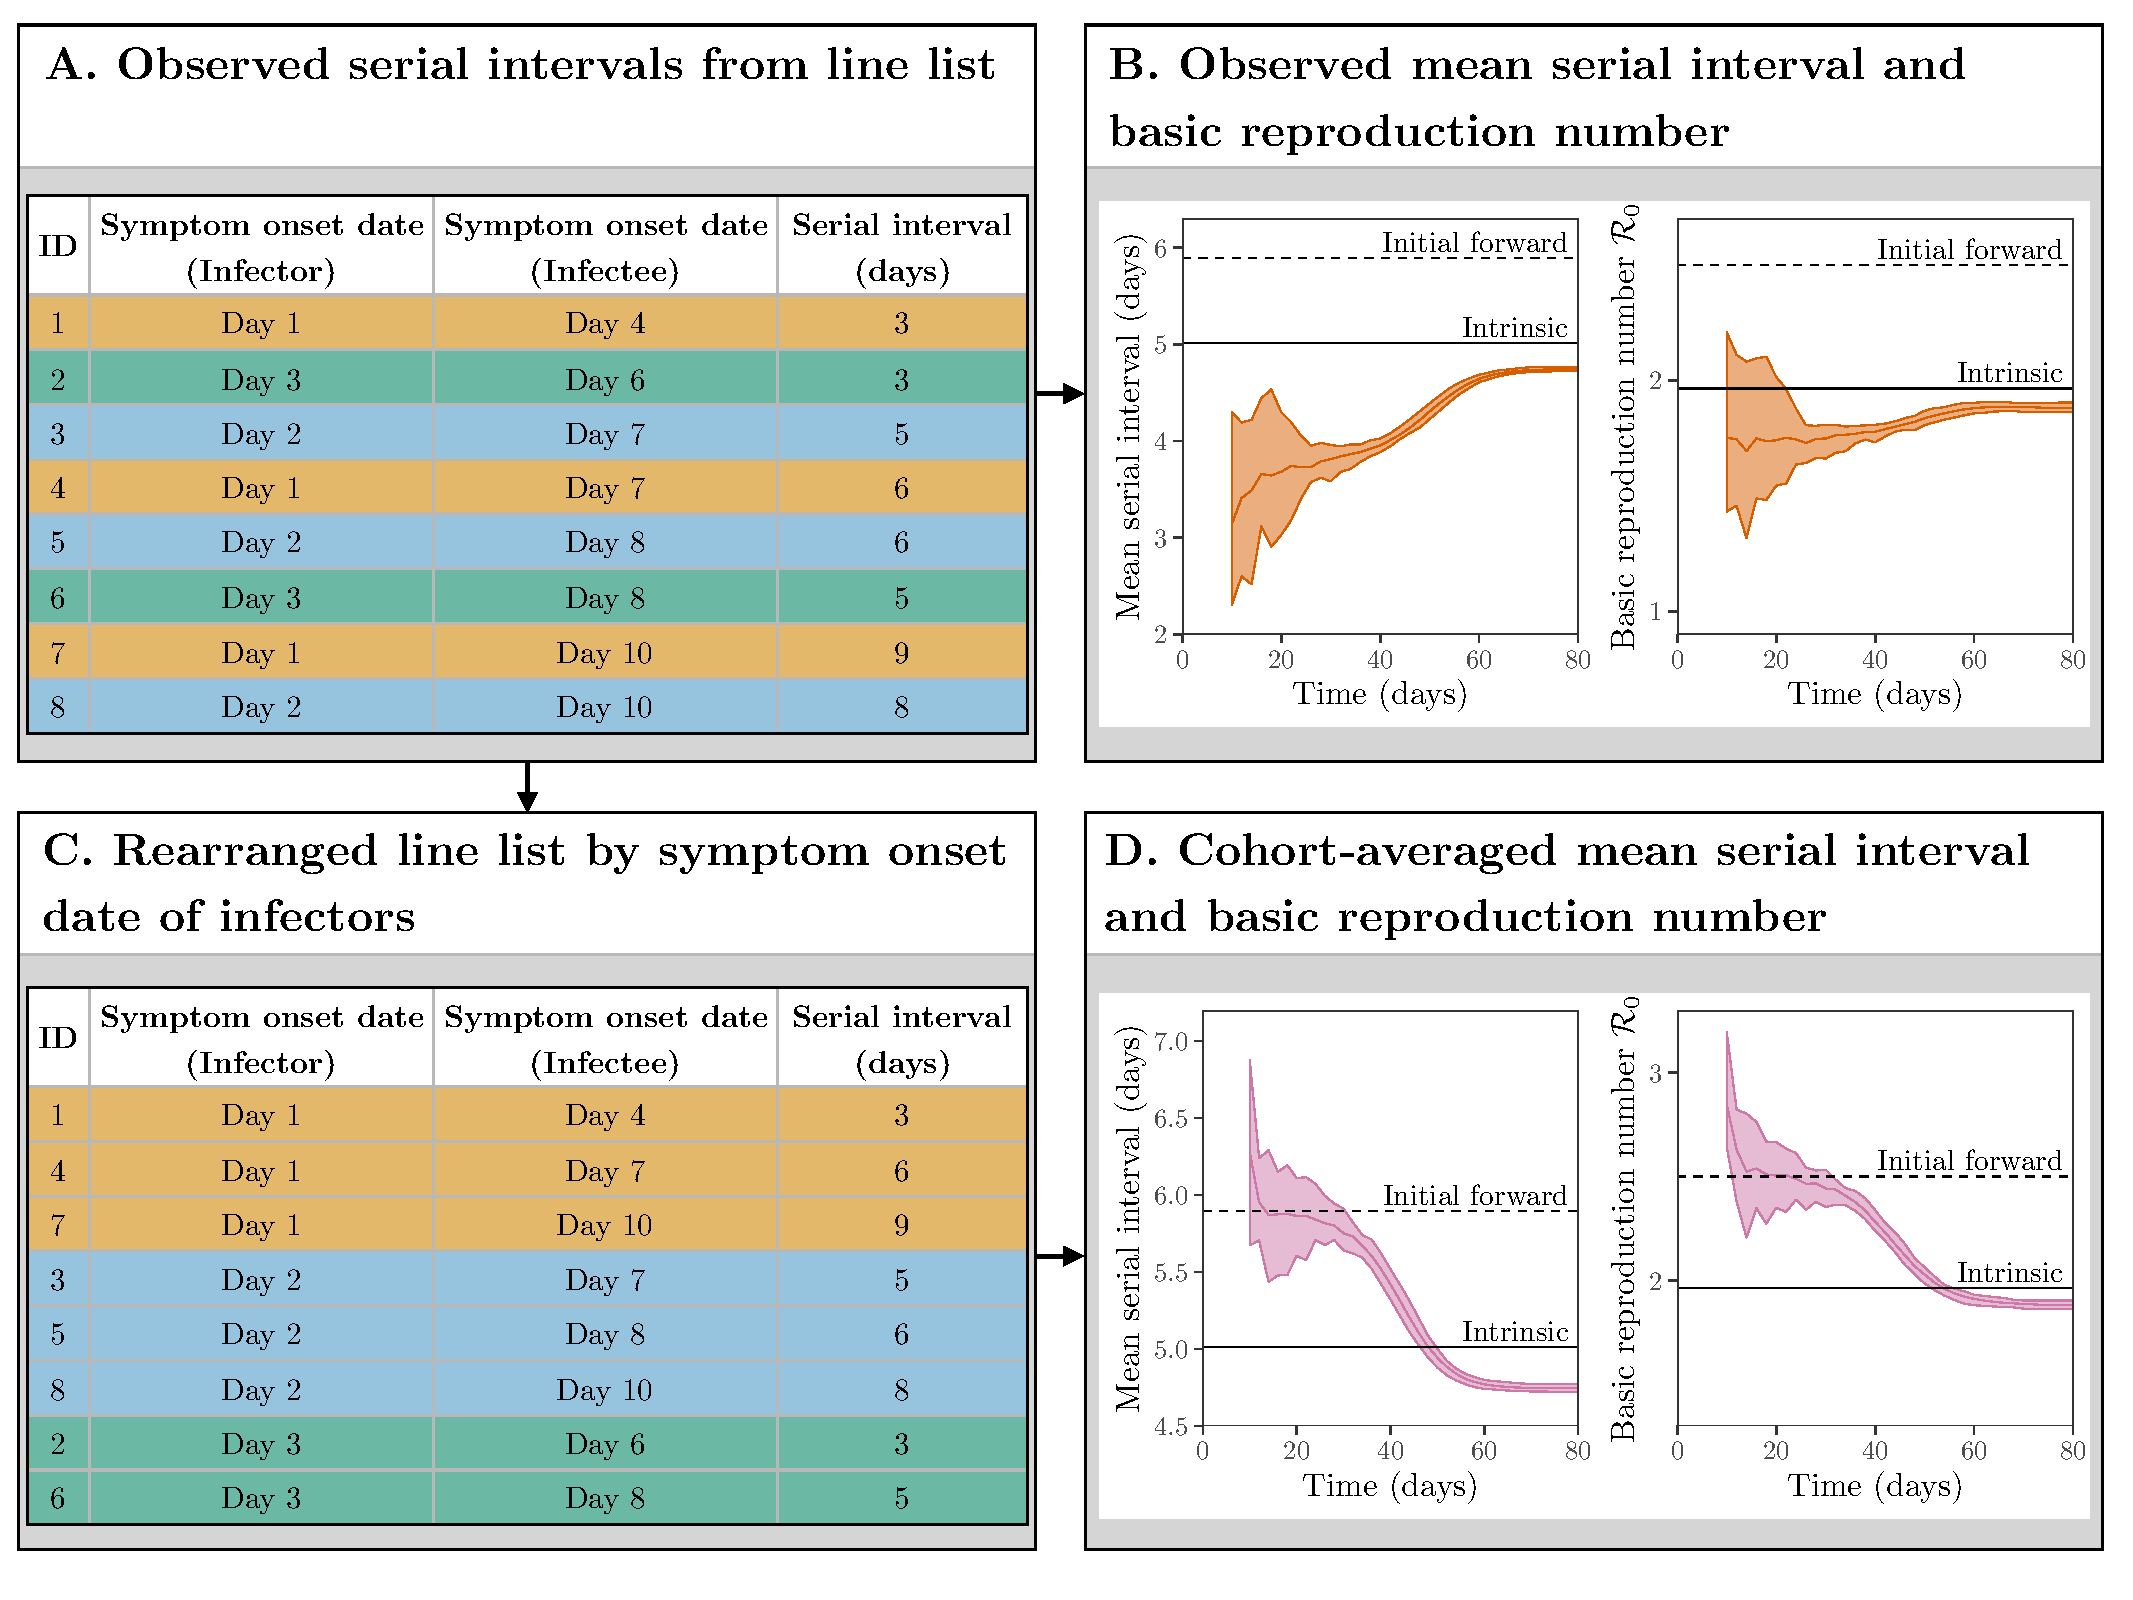
\includegraphics[width=\textwidth]{diagram.pdf}
\caption{
\textbf{Estimating the reproduction number from the observed serial intervals.}
(A) Schematic representation of line list data collected during an epidemic.
(B) Estimates of \Ro based on all observed serial intervals completed by a given time.
(C) Schematic representation of line list data rearranged by symptom onset date of infectors.
(D) Estimates of \Ro based on all observed serial intervals started by a given time. 
Black dashed lines represent the mean initial forward serial interval and \Ro.
Black solid lines represent the mean intrinsic serial interval and \Rintrinsic.
Colored solid lines represent the mean estimates of \Ro across 10 stochastic simulations.
Colored ribbons represent the range of estimates of \Ro across 10 stochastic simulations.
}
\label{fig:obsrR}
\end{figure}

Now\DIFaddbegin \DIFadd{, }\DIFaddend we turn to \DIFdelbegin \DIFdel{practical issues }\DIFdelend \DIFaddbegin \DIFadd{issues of estimating the reproduction number from the observed serial interval data during on ongoing epidemic}\DIFaddend .
In order to have an unbiased estimate of \DIFdelbegin %DIFDELCMD < \Ro%%%
\DIFdelend \DIFaddbegin \DIFadd{the basic reproduction number}\DIFaddend , we need to use serial-interval distributions estimated based on primary cohorts (i.e., infectors who share the same symptom onset time) at the early stage of the epidemic (i.e., initial forward serial-interval distribution).
However, \DIFdelbegin \DIFdel{when }\DIFdelend \DIFaddbegin \DIFadd{researchers typically use all available information to estimate epidemiological parameters;
in particular, \mbox{%DIFAUXCMD
\citep{thompson2019improved} }\hspace{0pt}%DIFAUXCMD
recently suggested that up-to-date serial interval data is necessary to accurately estimate the reproduction number.
We explore the consequences of neglecting changes in the realized serial interval distributions on estimates of the basic reproduction number.
}

\DIFadd{When }\DIFaddend an epidemic is ongoing, the observed serial intervals are subject to right-censoring because we cannot observe a serial interval if either an infector or an infectee has not yet developed symptoms;
for example, if we were to measure serial intervals on Day 8 as in \fref{obsrR}A, we will only be able to observe the first 6 events (ID 1--6).
\fref{obsrR}B demonstrates how the effect of right-censoring in the observed serial intervals translates to the underestimation of the basic reproduction number \Ro in our stochastic simulations \DIFaddbegin \DIFadd{(assuming $\Ro = 2.5$ as in \fref{epi})}\DIFaddend .
Notably, even if we could observe, and average, \emph{all} serial intervals across all transmission pairs after the epidemic has ended, we would still underestimate the initial mean forward serial interval (and therefore \Ro), likely by a large amount, because the observed serial-interval distribution converges to the intrinsic serial-interval distribution;
in fact, we would even underestimate the intrinsic value slightly due to contraction of the forward generation-interval distribution during the susceptible depletion phase (\fref{epi}C).

Here we provide a heuristic way of assessing potential biases in the estimate of the mean initial forward serial interval and therefore \Ro retrospectively.
\DIFdelbegin \DIFdel{Once serial intervals have been observed after the epidemic has been sufficiently progressed, we }\DIFdelend \DIFaddbegin \DIFadd{We }\DIFaddend can rearrange the line list and group observed serial intervals based on the symptom onset date of infectors (\fref{obsrR}C).
Then, we can compare how estimates of the mean serial interval as well as \Ro change as we incorporate more recent cohorts into the analysis;
that is, we analyze observed serial intervals from infectors who became symptomatic before time $t$ and evaluate how the estimates change as we increase $t$.
This approach is analogous to averaging over a set of forward intervals, just as using all information up to a certain time is analogous to averaging over a set of backward intervals (\fref{obsrR}D).
During the exponential growth phase, the estimates of the mean serial interval and \Ro are consistent with the \DIFdelbegin \DIFdel{target value }\DIFdelend \DIFaddbegin \DIFadd{true value (see `initial forward' in \fref{obsrR}B,D)}\DIFaddend ;
adding more data allows us to make more precise inference during this period.
However, the cohort-averaged estimates decrease rapidly soon after the exponential growth period, reflecting changes in the forward serial-interval distributions.
This approach allows us to detect dynamical changes in the forward serial-interval distributions and its effect on the estimates of \Ro.

\DIFaddbegin \subsection{\DIFadd{Applications to the COVID-19 pandemic}}

\DIFaddend \begin{figure}[!th]
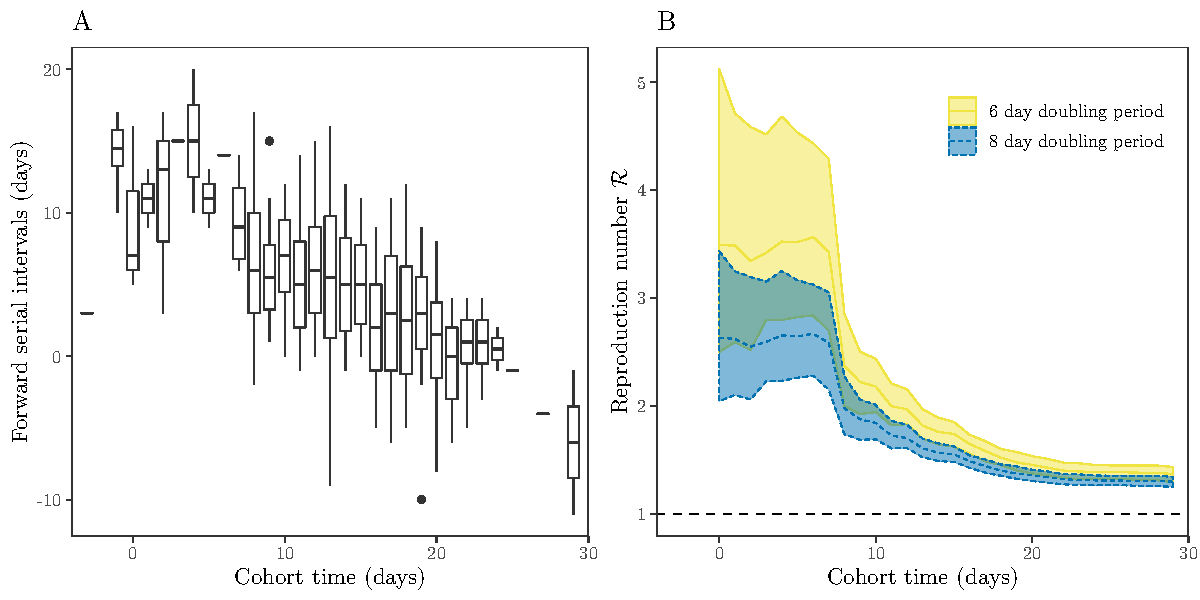
\includegraphics[width=\textwidth]{serial_analysis.pdf}
\caption{
\textbf{Observed serial intervals of COVID-19 and cohort-averaged estimates of \RR.}
(A--B) forward and backward serial intervals over time.
Points represent the means. 
Vertical error bars represent the 95\% equi-tailed quantiles.
Solid lines represent the estimated locally estimated scatterplot smoothing (LOESS) fits.
The dashed line represents the maximum and minimum observable delays across the range of .
(C) Cohort-averaged estimates of \Ro assuming doubling period of 6 and 8 days \citep{li2020early, wu2020nowcasting}.
Ribbons represent the associated 95\% bootstrap confidence intervals.
The data were taken from Supplementary Materials of \cite{du2020serial}.
}
\label{fig:du}
\end{figure}

\DIFdelbegin \subsection{\DIFdel{Applications to the COVID-19 pandemic}}
%DIFAUXCMD
\addtocounter{subsection}{-1}%DIFAUXCMD
%DIFDELCMD < 

%DIFDELCMD < %%%
\DIFdelend Finally, we re-analyze serial intervals of COVID-19 collected by \cite{du2020serial} from mainland China, outside Hubei province, based on transmission events reported between January 21--February 8, 2020;
\cite{du2020serial} estimated the mean serial \DIFaddbegin \DIFadd{interval }\DIFaddend of 3.96 days (95\% CI 3.53–4.39 days) and \Ro of 1.32 (95\% CI 1.16–1.48).
\fref{du}A shows that the mean forward serial interval decreases over time.
While the decrease is likely to be affected by the right-censoring (indicated by the closeness between the quantiles of the observed serial intervals and \emph{maximum observable} serial intervals), increase in the proportion of negative serial intervals are clearly indicative of the changes in the forward serial-interval distribution;
increase in the proportion of negative serial intervals is unlikely to be driven by the left-censoring (indicated by the ``farness'' between the quantiles of the observed serial intervals and \emph{minimum observable} serial intervals).
The decrease in the mean forward serial interval was likely to be caused by increase in the mean backward incubation periods, reflecting decrease in COVID-19 cases in China, as well as intervention efforts which reduce generation intervals by preventing infections once cases are identified.
\fref{du}B shows that the mean backward serial interval increases over time, also reflecting decrease in COVID-19 cases in China.

While the qualitative changes in the mean forward and backward serial interval are consistent with our earlier simulations (\fref{epi}), the initial mean forward serial interval (\fref{du}A) appears to be larger than what we calculate earlier based on previously estimated incubation period and generation-interval distributions (\fref{rR}C).
These results indicate that previous estimates of incubation period and generation-intervals (Table 1) may have been underestimated as neither study explicitly accounts for the fact that the observed distributions are like backward distributions.

\fref{du}C shows the cohort-averaged estimates of \Ro, which remain roughly constant until day 7 and suddenly decreases;
this sudden decrease is indicative of changes in the forward serial intervals as shown in our simulation study (\fref{obsrR}).
The \DIFaddbegin \DIFadd{cohort-averaged }\DIFaddend estimates of \Ro based on the early forward serial intervals are also consistent with previous estimates of \Ro of the COVID-19 epidemic in China \citep{majumder2020early, park2020reconciling}\DIFdelbegin \DIFdel{.
We note that }\DIFdelend \DIFaddbegin \DIFadd{:
$\Ro = 2.6$ (95\% CI: 2.2--3.1) and $\Ro = 3.4$ (95\% CI: 2.7 -- 4.3) based on 8 and 6 doubling periods, respectively, using serial interval data from infectors who developed symptoms by day 7.
These }\DIFaddend early cohort-averaged estimates of \Ro are unlikely to be affected by the right-censoring as we expect the degree of right-censoring to be low (\fref{du}A).
\DIFaddbegin \DIFadd{Therefore, }\Ro \DIFadd{estimate of 1.32 (95\% CI 1.16–1.48), which neglects the changes in the forward serial-interval distribution, is likely to be an underestimate.
}\DIFaddend This example demonstrates the danger of using the observed serial intervals to calculate the \DIFdelbegin \DIFdel{basic }\DIFdelend reproduction number without integrating serial intervals into cohorts.

\section{Discussion}

Generation and serial intervals determine the time scale of disease transmission, and are therefore critical to dynamical modeling of infectious outbreaks.
Here, we show that the initial \emph{forward} serial-interval distribution --- measured during the exponential growth phase of an epidemic --- provides the correct link between the exponential growth rate $r$ and the reproduction number \RR.
In general, \DIFdelbegin \DIFdel{this }\DIFdelend \DIFaddbegin \DIFadd{the forward serial-interval distributions }\DIFaddend will not match the intrinsic or the backward \DIFdelbegin \DIFdel{serial interval}\DIFdelend \DIFaddbegin \DIFadd{serial-interval distributions}\DIFaddend .
Further, \DIFdelbegin \DIFdel{this }\DIFdelend \DIFaddbegin \DIFadd{the mean forward serial }\DIFaddend interval can decrease over time due to disease dynamics. 
Failing to account for these differences can result in underestimation of \RR.

Our study underlines the importance of carefully defining measured epidemiological time distributions.
Previous studies have shown that generation interval can be either measured forward or backward \citep{nishiura2010time,champredon2015intrinsic,britton2019estimation};
we generalize these ideas and show that they apply to other epidemiological distributions.
Changes in the backward delay distributions due to changing cohort sizes is expected to be a pervasive feature of outbreak dynamics.
Recent analyses of COVID-19 epidemics have attempted to reconstruct epidemic time series of symptomatic cases or infected cases from the reports of confirmed cases by using time-independent delay distributions from infection or symptom onset to reporting (e.g., \cite{tempvar, park2020potential, shim2020transmission});
these studies effectively assume constant backward delay distributions.
Although such approaches may be able to roughly match the time scale of an epidemic, we recommend using dynamical approaches that model incidence as well as reporting delays explicitly (e.g., \citep{flaxman2020estimating}).

While our results support the use of serial interval distributions for calculating \RR, 
they also reveal gaps in current practices in incorporating serial-interval distributions into outbreak analyses.
\DIFdelbegin \DIFdel{In particular, }\DIFdelend \cite{thompson2019improved} recently emphasized the importance of using up-to-date serial interval data for accurate estimation of time-varying reproduction numbers\DIFdelbegin \DIFdel{;
however}\DIFdelend \DIFaddbegin \DIFadd{.
However}\DIFaddend , our study demonstrates that early serial interval data is required to estimate \DIFaddbegin \DIFadd{the initial }\DIFaddend \RR \DIFaddbegin \DIFadd{during the exponential growth phase }\DIFaddend and that using up-to-date serial interval data (without accounting for changes in the forward serial-interval distribution) can, in fact, underestimate \DIFaddbegin \DIFadd{the initial }\DIFaddend \RR.
\DIFaddbegin \DIFadd{Future studies should explore how neglecting changes in the forward serial-interval distribution can affect the estimates of }\RR \DIFadd{beyond the exponential growth phase and potentially re-asses existing estimates of }\RR\DIFadd{.
}

\DIFaddend Many studies have already estimated the (time-varying) reproduction numbers for COVID-19 epidemics using aggregated serial interval data (e.g., \cite{tempvar,du2020serial,pan2020jama,zhang2020evolving});
these studies should \DIFaddbegin \DIFadd{also }\DIFaddend re-assess whether they appropriately considered the \emph{forward} serial interval.
Given large geographical \DIFdelbegin \DIFdel{differences in the observed exponential growth rates }\DIFdelend \DIFaddbegin \DIFadd{variation in the spread }\DIFaddend of the COVID-19\DIFdelbegin \DIFdel{epidemic, the initial }\DIFdelend \DIFaddbegin \DIFadd{, the }\DIFaddend forward serial interval distributions are also likely to vary across different countries.
We suggest that modelers should aim to characterize spatiotemporal variation in \DIFdelbegin \DIFdel{initial }\DIFdelend forward serial-interval distributions and understand their changes over time.
These modeling approaches should be necessarily coupled with intensive epidemiological investigation through contact tracing at the very beginning of the outbreak in order to characterize the initial forward serial-interval distribution, particularly for an emerging epidemic such as COVID-19.

Our study also underlines the fact that the serial-interval distribution depends not only on the generation-interval and incubation-period distributions, but also on their intrinsic correlations.
This implies that not considering this correlation can bias the estimates of the intrinsic generation-interval distribution from the serial-interval distribution.
Furthermore, previous studies that tried to estimate the generation-interval distributions from the observed serial intervals often ignored the dynamical differences between the realized incubation periods of infectors (backward-looking) and those of infectees (forward looking) (e.g., \cite{klinkenberg2011correlation, ganyani2020estimating}).
There is currently a need for better statistical tools for teasing apart the intrinsic generation-interval distributions from the observed serial intervals.

Our study is not without limitations.
We assumed that all individuals develop symptoms and that the the entire transmission process, including all relevant epidemiological delays, are known exactly.
In practice, asymptomatic and presymptomatic transmission of COVID-19 makes measuring serial intervals difficult \citep{bai2020presumed,he2020temporal,wei2020presymptomatic}.
Biases in the observed serial intervals will necessarily bias the estimates of \RR. 
Furthermore, serial intervals do not take into account asymptomatic transmission; 
not explicitly accounting for asymptomatic transmission may also bias the estimates of \RR \citep{park2020time}.

While we focused on the effect of epidemiological dynamics on the serial-interval distributions, other factors, such as intervention strategies, can also affect the generation- and serial-interval distributions.
Individual-level interventions, such as case isolation, directly affect individuals' ability to transmit and will shorten the forward generation- and serial-intervals.
Population-level interventions, such as social distancing, can squeeze contacts into household and introduce high degree of clustering, which, in turn, will shorten the realized generation intervals due to local depletion of the susceptible pool within households \citep{park2019inferring}.

Despite these limitations, our analysis of serial intervals of COVID-19 from China provide further support for our theoretical framework, demonstrating temporal variation in serial intervals and their effects on the estimates of \RR.
To our knowledge, most existing estimates of the serial-intervals of COVID-19 implicitly or explicitly assume that the serial-interval distributions remain constant throughout the course of an epidemic \citep{du2020serial, he2020temporal, nishiura2020serial,tindale2020transmission,zhao2020estimating,zhang2020evolving}.
Our study provides a rationale for reassessing estimates of serial-interval distributions, and their use in estimating \RR, of the COVID-19 pandemic.

\pagebreak

\section{\DIFdelbegin \DIFdel{Appendix}\DIFdelend \DIFaddbegin \DIFadd{Supplementary Materials}\DIFaddend }

\subsection{Deterministic simulation}

We simulate the renewal equation model using a discrete-time approximation:
\begin{equation}
\DIFdelbegin %DIFDELCMD < \begin{aligned}
%DIFDELCMD < i(t) &= \Ro S(t-\Delta t) \sum_{m=1}^{\ell} i(t-m \Delta t) \hat{\gdist}(m \Delta t) \\
%DIFDELCMD < S(t) &= S(t-\Delta t) - i(t)
%DIFDELCMD < \end{aligned}%%%
\DIFdelend \DIFaddbegin \begin{aligned}
i(t) &= \Ro S(t-\Delta t) \sum_{m=1}^{\tsub{m}{max}} i(t-m \Delta t) \hat{\gdist}(m \Delta t) \\
S(t) &= S(t-\Delta t) - i(t)
\end{aligned}\DIFaddend 
\end{equation}
where $\hat{\gdist}$ is a discrete-time intrinsic generation-interval distribution that satisfies the following:
\begin{equation}
\hat{\gdist}(m \Delta t) = \frac{\gdist(m \Delta t)}{\sum_{i=1}^\ell \gdist(m \Delta t)}, \quad m=1, \dots, \DIFdelbegin \DIFdel{\ell
}\DIFdelend \DIFaddbegin \tsub{m}{max}\DIFadd{.
}\DIFaddend \end{equation}
The continuous-time intrinsic generation-interval distribution is parameterized using a log-normal distribution (Table 1). We define the \DIFdelbegin \DIFdel{forward }\DIFdelend \DIFaddbegin \DIFadd{intrinsic }\DIFaddend incubation period distribution in a similar manner:
\begin{equation}
\DIFdelbegin %DIFDELCMD < \hat{k}%%%
\DIFdelend \DIFaddbegin \hat{\idist}\DIFaddend (m \Delta t) = \DIFdelbegin \DIFdel{\frac{k(m \Delta t)}{\sum_{i=1}^\ell k(m \Delta t)}}\DIFdelend \DIFaddbegin \DIFadd{\frac{\idist(m \Delta t)}{\sum_{i=1}^\ell \idist(m \Delta t)}}\DIFaddend , \quad m=1, \dots, \DIFdelbegin \DIFdel{\ell}\DIFdelend \DIFaddbegin \tsub{m}{max}\DIFaddend ,
\end{equation}
where its continuous-time analog is also based on a log-normal distribution.
For \DIFdelbegin \DIFdel{brevity}\DIFdelend \DIFaddbegin \DIFadd{simplicity}\DIFaddend , we assume that the forward incubation periods and intrinsic generation intervals are independent:
\begin{equation}
\hat{h}(m \Delta t, \DIFaddbegin \DIFadd{n }\DIFaddend \Delta t\DIFdelbegin \DIFdel{n}\DIFdelend ) = \DIFdelbegin %DIFDELCMD < \hat{k}%%%
\DIFdelend \DIFaddbegin \hat{\idist}\DIFaddend (m \Delta t)\hat{\gdist}(\DIFaddbegin \DIFadd{n }\DIFaddend \Delta t\DIFdelbegin \DIFdel{n}\DIFdelend ), \quad m,n=1, \dots, \DIFdelbegin \DIFdel{\ell}\DIFdelend \DIFaddbegin \tsub{m}{max}\DIFaddend .
\end{equation}
We use $\Delta t = 0.025\,\textrm{days}$ and \DIFdelbegin \DIFdel{$\ell=2001$ }\DIFdelend \DIFaddbegin \DIFadd{$\tsub{m}{max}=2001$ }\DIFaddend for discretization steps.

We initialize the simulation with population size $N$=40,000 as follows:
\begin{equation}
\DIFdelbegin %DIFDELCMD < \begin{aligned}
%DIFDELCMD < i(m \Delta t) &= C \exp(r m \Delta t), \quad m=1, \dots, \ell\\
%DIFDELCMD < S(m \Delta t) &= N - \sum_{n=1}^m i(m \Delta t), \quad m=1, \dots, \ell\\
%DIFDELCMD < \end{aligned}%%%
\DIFdelend \DIFaddbegin \begin{aligned}
i(m \Delta t) &= C \exp(r m \Delta t), \quad m=1, \dots, \tsub{m}{max}\\
S(m \Delta t) &= N - \sum_{n=1}^m i(n \Delta t), \quad m=1, \dots, \tsub{m}{max}\\
\end{aligned}\DIFaddend 
\end{equation}
where $C$ is chosen such that \DIFdelbegin \DIFdel{$\sum_{n=1}^\ell i(m \Delta t)=10$}\DIFdelend \DIFaddbegin \DIFadd{$\sum_{n=1}^{\tsub{m}{max}} i(m \Delta t)=10$}\DIFaddend .
These initial conditions allow the model to follow exponentially growth from time \DIFdelbegin \DIFdel{$\Delta t (\ell + 1)$ }\DIFdelend \DIFaddbegin \DIFadd{$\Delta t (\tsub{m}{max} + 1)$ }\DIFaddend without any transient behaviors.
Results presented in the main text show simulations beginning from time \DIFdelbegin \DIFdel{$\Delta t (\ell + 1)$}\DIFdelend \DIFaddbegin \DIFadd{$\Delta t (\tsub{m}{max} + 1)$}\DIFaddend .

\subsection{Stochastic simulation}

We run stochastic simulations of the renewal equation model using an individual-based model on a fully connected network (i.e., homogeneous population) based on the Gillespie algorithm that we developed earlier \citep{park2019inferring}.
First, we initialize an epidemic with $I(0)$ infected individuals (nodes) in a fully connected network of size $N$. 
For each initially infected individual, we draw number of infectious contacts from a Poisson distribution with the mean of \Ro and the corresponding generation intervals for each contact from a log-normal distribution (Table 1).
Contactees are uniformly sampled from the total population.
All contactees are sorted into event queues based on their infection time.
We update the current time to the infection time of the first person in the queue.
Then, the first person in the queue makes contacts based on the Poisson offspring distribution described earlier and their contactees are added to the sorted queue.
Whenever contactees are added to the sorted queue, we remove all duplicated contacts (but keep the first one) as well as contacts made to individuals that have already been infected.
Simulations continue until there are no more individuals in the queue.
We simulate 10 epidemics with $I(0)=10$ and $N$=40,000.

\subsection{Linking $r$ and \Ro using serial-interval distributions}

The intrinsic generation-interval distribution $\gdist(\tau)$ provides a link between $r$ and \Ro via the Euler-Lotka equation:
\begin{equation}
\frac{1}{\Ro} = \int_0^\infty \exp(-r\tau) \gdist(\tau) \dtau.
\end{equation}
Here, we prove that the initial forward serial-interval distribution $f_0$ also provides the same link:
\begin{equation}
\frac{1}{\Ro} = \int_{-\infty}^\infty \exp(-r\tau) f_{0}(\tau) \dtau,
\end{equation}
where the initial forward serial-interval distribution is defined as:
\begin{equation}
f_{0}(\tau) \propto \int_{-\infty}^{0} \int_{\alpha_1}^{\tau} \exp(r \alpha_1) h(-\alpha_1, \alpha_2 - \alpha_1) \DIFdelbegin \DIFdel{k}\DIFdelend \DIFaddbegin \DIFadd{\idist}\DIFaddend (\tau - \alpha_2) \, \mathrm{d}\alpha_2\,\mathrm{d}\alpha_1.
\end{equation}

First, we rewrite the initial forward serial-interval distribution in the following form:
\begin{equation}
\DIFdelbegin %DIFDELCMD < \begin{aligned}
%DIFDELCMD < f_{0}(\tau) &\propto \int_0^\infty \int_{-\pinf}^{\tau} \exp(-r\pinf) h(\pinf, \sinf + \pinf) k(\tau - \sinf) \mathrm{d}\sinf\,\mathrm{d}\pinf\\
%DIFDELCMD < &= \int_{-\infty}^{\tau} \int_{\max{(0,-\sinf)}}^{\infty} \exp(-r\pinf) h(\pinf, \sinf + \pinf)k(\tau - \sinf)\mathrm{d}\pinf\, \mathrm{d}\sinf\\
%DIFDELCMD < \end{aligned}%%%
\DIFdelend \DIFaddbegin \begin{aligned}
f_{0}(\tau) &\propto \int_0^\infty \int_{-\pinf}^{\tau} \exp(-r\pinf) h(\pinf, \sinf + \pinf) \idist(\tau - \sinf) \mathrm{d}\sinf\,\mathrm{d}\pinf\\
&= \int_{-\infty}^{\tau} \int_{\max{(0,-\sinf)}}^{\infty} \exp(-r\pinf) h(\pinf, \sinf + \pinf)\idist(\tau - \sinf)\mathrm{d}\pinf\, \mathrm{d}\sinf\\
\end{aligned}\DIFaddend 
\end{equation}
It follows that $z(\sinf)$ describes the time between symptom onset of infector and infection of infectee:
\begin{equation}
z(\sinf) \propto \int_{\max{(0,-\sinf)}}^{\infty} \exp(-r\pinf) h(\pinf, \sinf + \pinf) \mathrm{d}\pinf.
\end{equation}
The initial forward serial-interval distribution $f_0$ can be expressed as a convolution of $z$ and \DIFdelbegin \DIFdel{$k$:
}\DIFdelend \DIFaddbegin \DIFadd{$\idist$:
}\DIFaddend \begin{equation}
\DIFdelbegin %DIFDELCMD < \begin{aligned}
%DIFDELCMD < f_{0}(\tau) &\propto \int_{-\infty}^{\tau} z(\sinf) k(\tau - \sinf) \mathrm{d}\sinf.\\
%DIFDELCMD < \end{aligned}%%%
\DIFdelend \DIFaddbegin \begin{aligned}
f_{0}(\tau) &\propto \int_{-\infty}^{\tau} z(\sinf) \idist(\tau - \sinf) \mathrm{d}\sinf.\\
\end{aligned}\DIFaddend 
\end{equation}
Then, we have
\begin{equation}
\int_{-\infty}^\infty \exp(-r\tau) f_{0}(\tau) \mathrm{d} \tau = \int_{-\infty}^\infty \exp(-r\tau) z(\tau) \mathrm{d} \tau \int_{0}^\infty \exp(-r\tau) \DIFdelbegin \DIFdel{k}\DIFdelend \DIFaddbegin \DIFadd{\idist}\DIFaddend (\tau) \mathrm{d} \tau
\end{equation}

Note that 
\begin{equation}
\DIFdelbegin %DIFDELCMD < \begin{aligned}
%DIFDELCMD < &\int_{-\infty}^\infty \int_{\max{(0,-\sinf)}}^{\infty} \exp(-r\pinf) h(\pinf, \sinf + \pinf) \mathrm{d}\pinf \mathrm{d}\sinf\\
%DIFDELCMD < &= \int_{0}^\infty \int_{-\pinf}^\infty \exp(- r \pinf) h(\pinf, \sinf+\pinf) \mathrm{d}\sinf\,\mathrm{d} \pinf\\
%DIFDELCMD < &= \int_{0}^\infty \exp(- r \pinf) k(\pinf) d\pinf
%DIFDELCMD < \end{aligned}%%%
\DIFdelend \DIFaddbegin \begin{aligned}
&\int_{-\infty}^\infty \int_{\max{(0,-\sinf)}}^{\infty} \exp(-r\pinf) h(\pinf, \sinf + \pinf) \mathrm{d}\pinf \mathrm{d}\sinf\\
&= \int_{0}^\infty \int_{-\pinf}^\infty \exp(- r \pinf) h(\pinf, \sinf+\pinf) \mathrm{d}\sinf\,\mathrm{d} \pinf\\
&= \int_{0}^\infty \exp(- r \pinf) \idist(\pinf) d\pinf
\end{aligned}\DIFaddend 
\end{equation}
because \DIFdelbegin \DIFdel{$k$ }\DIFdelend \DIFaddbegin \DIFadd{$\idist$ }\DIFaddend is a marginal probability distribution of $h$.
Since \DIFdelbegin \DIFdel{$\int_{0}^\infty \exp(- r \pinf) k(\pinf) d\pinf$ }\DIFdelend \DIFaddbegin \DIFadd{$\int_{0}^\infty \exp(- r \pinf) \idist(\pinf) d\pinf$ }\DIFaddend is a normalization factor for probability distribution $z$, we have:
\begin{equation}
\int_{-\infty}^\infty \exp(-r\tau) z(\tau) \mathrm{d} \tau = \DIFdelbegin \DIFdel{\frac{\int_{-\infty}^\infty \exp(-r\tau) \int_{\max{(0,-\sinf)}}^{\infty} \exp(-r\pinf) h(\pinf, \sinf + \pinf) \mathrm{d}\pinf \mathrm{d}\tau}{\int_{0}^\infty \exp(- r \pinf) k(\pinf) d\pinf}}\DIFdelend \DIFaddbegin \DIFadd{\frac{\int_{-\infty}^\infty \exp(-r\tau) \int_{\max{(0,-\sinf)}}^{\infty} \exp(-r\pinf) h(\pinf, \sinf + \pinf) \mathrm{d}\pinf \mathrm{d}\tau}{\int_{0}^\infty \exp(- r \pinf) \idist(\pinf) d\pinf}}\DIFaddend .
\end{equation}
Then, we have:
\begin{equation}
\int_{-\infty}^\infty \exp(-r\tau) f_{0}(\tau) \mathrm{d} \tau = \int_{-\infty}^\infty \exp(-r\tau) \int_{\max{(0,-\sinf)}}^{\infty} \exp(-r\pinf) h(\pinf, \sinf + \pinf) \mathrm{d}\pinf \mathrm{d}\tau.
\end{equation}

We are left to show that 
\begin{equation}
\int_0^{\infty} \exp(-r\tau) g(\tau) \mathrm{d}\tau = \int_{-\infty}^\infty \exp(-r\tau) \int_{\max{(0,-\sinf)}}^{\infty} \exp(-r\pinf) h(\pinf, \sinf + \pinf) \mathrm{d}\pinf \mathrm{d}\tau,
\end{equation}
where the intrinsic generation-interval distribution $g$ is also a marginal probability distribution of $f$:
\begin{equation}
g(\tau) = \int_0^\infty h(\pinf, \tau)  \mathrm{d} \pinf.
\end{equation}
Let $\sigma = \pinf + \tau$. Then, by change of variables, it immediately follows that
\begin{equation}
\begin{aligned}
&\int_{-\infty}^{\infty} \exp(-r\tau) \int_{\max(0, -\tau)}^\infty \exp(- r \pinf) h(\pinf, \tau+\pinf) \mathrm{d} \pinf\, \mathrm{d}\tau\\
&=\int_{0}^{\infty} \int_{0}^\infty \exp(- r \sigma) h(\pinf, \sigma) \mathrm{d} \pinf\, \mathrm{d}\sigma\\
&=\int_{0}^{\infty} \exp(-r\tau) g(\tau) \mathrm{d}\tau
\end{aligned}
\end{equation}
Therefore, the initial forward serial--interval distribution and the intrinsic generation-interval distribution give the same link between $r$ and \RR.

\subsection{Comparing the estimates of \Ro using the initial forward and the intrinsic serial-interval distributions}

We use a simulation-based approach to compare the estimates of \Ro based on the serial- and generation-interval distributions. 
To do so, we model the intrinsic generation-interval distribution and the incubation period using a multivariate log-normal distribution with log means $\mu_G, \mu_I$, log standard variances $\sigma_G^2, \sigma_I^2$, and log-scale correlation $\rho$;
the multivariate log-normal distribution is parameterized based on parameter estimates for COVID-19 (Table 1).
We construct forward serial intervals during the exponential growth period as follows:
\begin{equation}
F_i = -X\DIFdelbegin \DIFdel{_{0,i} }\DIFdelend \DIFaddbegin \DIFadd{_{1,i} }\DIFaddend + (G_i|X\DIFdelbegin \DIFdel{_{0,i}}\DIFdelend \DIFaddbegin \DIFadd{_{1,i}}\DIFaddend ) + X\DIFdelbegin \DIFdel{_{1,i}}\DIFdelend \DIFaddbegin \DIFadd{_{2,i}}\DIFaddend ,
\end{equation}
where the backward incubation period \DIFdelbegin \DIFdel{$X_{0,i}$ }\DIFdelend \DIFaddbegin \DIFadd{$X_{1,i}$ }\DIFaddend of an infector is simulated by drawing random log-normal samples $Y_i$ with log mean $\mu_I$ and log variance $\sigma_I^2$ and resampling $Y_i$, each weighted by the inverse of the exponential growth function $\exp(-rY_i)$;
the intrinsic generation interval conditional on the incubation period of the infector \DIFdelbegin \DIFdel{$(G_i|X_{0,i})$ }\DIFdelend \DIFaddbegin \DIFadd{$(G_i|X_{1,i})$ }\DIFaddend is drawn from a log-normal distribution with log mean \DIFdelbegin \DIFdel{$\mu_G + \sigma_G \rho (\log(X_{0,i}) - \mu_I)/\sigma_I$ }\DIFdelend \DIFaddbegin \DIFadd{$\mu_G + \sigma_G \rho (\log(X_{1,i}) - \mu_I)/\sigma_I$ }\DIFaddend and log variance $\sigma_G^2 (1-\rho^2)$;
the forward incubation period \DIFdelbegin \DIFdel{$X_{1,i}$ }\DIFdelend \DIFaddbegin \DIFadd{$X_{2,i}$ }\DIFaddend of an infectee is drawn from a log-normal distribution with log mean $\mu_I$ and log variance $\sigma_I^2$.
We then calculate the basic reproduction number \Ro using the empirical estimator:
\begin{equation}
\Ro = \frac{1}{\frac{1}{N}\sum_{i=1}^N \exp(- r F_i)}.
\end{equation}
We compare this with an estimate of \Ro based on the intrinsic serial-interval distribution in which the backward and the forward incubation periods are identically distributed \citep{svensson2007note,klinkenberg2011correlation,champredon2018equivalence, britton2019estimation}:
\begin{equation}
  \Rintrinsic = \frac{1}{\frac{1}{N}\sum_{i=1}^N \exp(- r Q_i)},
\end{equation}
where
\begin{equation}
Q_i = -Y_i + (G_i|Y_i) + X\DIFdelbegin \DIFdel{_{1,i}}\DIFdelend \DIFaddbegin \DIFadd{_{2,i}}\DIFaddend .
\end{equation}

\subsection{Applications: SEIR model}

Consider a Susceptible-Exposed-Infectious-Recovered model:
\begin{equation}
\begin{aligned}
\frac{\mathrm{d}S}{\mathrm{d}t} &= - \beta S I\\
\frac{\mathrm{d}E}{\mathrm{d}t} &= \beta S I - \sigma E\\
\frac{\mathrm{d}I}{\mathrm{d}t} &= \sigma E - \gamma I \\
\frac{\mathrm{d}R}{\mathrm{d}t} &= \gamma I \\
\end{aligned}
\end{equation}
where $\beta$ is the transmission rate, $1/\sigma$ is the mean latent period, and $1/\gamma$ is the mean infectious period.
We further assume that the latent period is equivalent to incubation period; in other words, infected individuals can only transmit after symptom onset.
Then, the generation interval will be always longer than the incubation period.

The joint probability distribution of the intrinsic incubation periods and intrinsic generation intervals for this model can be written as:
\begin{equation}
h(x, \tau) = \begin{cases}
0 & x > \tau\\
\gamma \sigma \exp(-\gamma (\tau-x)-\sigma x) & x \leq \tau
\end{cases}
\end{equation}
Then, the intrinsic generation-interval distribution is given by:
\begin{equation}
\begin{aligned}
g(\tau) &= \int_0^\tau h(x, \tau) \dx\\
&= \frac{\gamma \sigma}{\sigma-\gamma} (\exp(-\gamma \tau) - \exp(-\sigma \tau))
\end{aligned}
\end{equation}
On the other hand, the initial forward serial-interval distribution is given by:
\begin{equation}
\begin{aligned}
f_{0}(\tau) &\propto \int_{-\infty}^{0} \int_{0}^{\tau} \exp(r \pinf) h(-\pinf, \sinf - \pinf) \idist(\tau - \sinf) \, \mathrm{d}\sinf\,\mathrm{d}\pinf\\
&\propto \int_{-\infty}^{0} \int_{0}^{\tau}\exp(r \pinf) \exp(-\gamma \sinf+ \sigma \pinf) \exp(-\sigma(\tau-\sinf)) \, \mathrm{d}\sinf\,\mathrm{d}\pinf\\
&\propto  \exp(-\sigma \tau) \int_{-\infty}^{0} \int_{0}^{\tau} \exp((\sigma-\gamma) \sinf) \exp((r+ \sigma) \pinf)\, \mathrm{d}\sinf\,\mathrm{d}\pinf\\
&\propto  (\exp(-\gamma \tau) - \exp(-\sigma \tau)) \int_{-\infty}^{0} \exp((r+ \sigma) \pinf)\,\mathrm{d}\pinf\\
&\propto  \exp(-\gamma \tau) - \exp(-\sigma \tau)
\end{aligned}
\end{equation}
Therefore, both the intrinsic generation intervals and the initial forward serial intervals are identically distributed and have the same mean.

\pagebreak

\bibliography{serial}

\end{document}
